\documentclass[12pt,a4paper]{article}
\usepackage[utf8]{inputenc}
\usepackage[spanish]{babel}
\usepackage{geometry}
\usepackage{amsmath}
\usepackage{amssymb}
\usepackage{booktabs}
\usepackage{longtable}
\usepackage{graphicx}
\usepackage{enumitem}
\usepackage{float}
\usepackage{xcolor}
\usepackage{fancyhdr}
\usepackage{caption}
\usepackage[numbers]{natbib}
\usepackage[colorlinks=true,linkcolor=black,citecolor=blue,urlcolor=blue]{hyperref}

\geometry{margin=2.5cm}

\pagestyle{fancy}
\fancyhf{}
\fancyhead[L]{T7 – Rejillas + Desarenador + ABR-RAP + BAF + Cloro + Lecho de Secado}
\fancyhead[R]{\thepage}

\setcounter{tocdepth}{2}

\begin{document}

\begin{titlepage}
\centering
\vspace*{2cm}

{\Huge\bfseries Memoria de Cálculo\par}
\vspace{1.5cm}

{\Large\itshape Dimensionamiento de:\par}
\vspace{0.5cm}

{\LARGE\bfseries T7 – Rejillas + Desarenador + ABR-RAP + BAF + Cloro + Lecho de Secado\par}
\vspace{2cm}

{\large Caudal de diseño: 17.31 L/s\par}
{\large Número de líneas: 3\par}
\vfill
{\large\today\par}
\end{titlepage}

\tableofcontents

\listoffigures

\listoftables

\newpage
\section{Resumen del Proyecto}

Este documento presenta el dimensionamiento detallado del T7 – Rejillas + Desarenador + ABR-RAP + BAF + Cloro + Lecho de Secado, disenado para tratar un caudal de 17.31 L/s distribuido en 3 lineas paralelas (5.77 L/s por linea).

\textbf{Caracteristicas del afluente:}
\begin{itemize}
    \item DBO$_5$: 243.1 mg/L
    \item DQO: 498.0 mg/L
    \item SST: 156.0 mg/L
    \item Coliformes fecales: 3e+03 NMP/100mL
    \item Temperatura: 25.6°C
\end{itemize}

\textbf{Secuencia de unidades del tren:} 
Canal de Desbaste con Rejillas $\rightarrow$ Desarenador de Flujo Horizontal $\rightarrow$ Reactor Anaerobio con Pantallas (ABR/RAP) $\rightarrow$ Biofiltro Biológico Aireado (BAF) $\rightarrow$ Sistema de Desinfeccion con Hipoclorito de Sodio $\rightarrow$ Lechos de Secado de Lodos

\newpage
\section{Dimensionamiento de Unidades}

\subsection{Canal de Desbaste con Rejillas}

\

Las rejillas constituyen la primera barrera de proteccion del sistema, reteniendo solidos gruesos como plasticos, ramas y papel que podrian danar equipos o causar obstrucciones en tuberias aguas abajo. El diseno hidraulico de esta unidad debe garantizar velocidades suficientes para arrastrar solidos sedimentables, pero no tan elevadas que dificulten el paso del agua a traves de las barras.

Segun los criterios establecidos por Metcalf y Eddy \cite{metcalf2014}, las velocidades de diseno en canales con rejillas deben mantenerse entre 0.40 y 0.60~m/s. Para este proyecto se adopta un valor intermedio de 0.50~m/s, lo cual resulta apropiado considerando el caudal de diseno. El tirante hidraulico se establece en 0.40~m, valor que permite una velocidad de flujo uniforme en la seccion del canal y evita la sedimentacion de solidos organicos antes de la rejilla, segun los criterios de Metcalf y Eddy \cite{metcalf2014}.

La perdida de carga en rejillas limpias se calcula mediante la formula de Kirschmer (1926), que relaciona la geometria de las barras con las caracteristicas del flujo. Los parametros que determinan esta perdida son: el espaciado entre barras ($b$), el espesor de las barras ($w$), la velocidad del flujo ($v$) y el angulo de inclinacion ($\theta$):

\begin{equation}
h_L = \beta \cdot \left(\frac{w}{b}\right)^{4/3} \cdot \frac{v^2}{2g} \cdot \sin\theta
\end{equation}
\captionequation{Perdida de carga en rejillas limpias - Formula de Kirschmer}

\textit{Donde:}
\begin{itemize}[noitemsep,leftmargin=2em]
    \item[$h_L$] = Perdida de carga en rejillas limpias (m)
    \item[$\beta$] = Factor de forma de la barra (2.42 para barras rectangulares)
    \item[$w$] = Espesor de la barra (10 mm)
    \item[$b$] = Espaciado entre barras (15 mm)
    \item[$v$] = Velocidad del flujo en el canal (m/s)
    \item[$g$] = Aceleracion de la gravedad (9,81 m/s\textsuperscript{2})
    \item[$\theta$] = Angulo de inclinacion de las barras (60\textdegree)
\end{itemize}

\begin{table}[H]
\centering
\caption{Parametros de diseno -- Rejillas}
\begin{tabular}{llcc}
\toprule
Parametro & Descripcion & Valor adoptado & Fuente \\
\midrule
Velocidad en canal & Velocidad de paso & 0.50 m/s & Metcalf y Eddy \\
Tirante hidraulico & Altura de agua en canal & 0.40 m & Criterio tecnico \\
Angulo de rejilla & Inclinacion barras & 60\textdegree & Practica comun \\
Espaciado entre barras & Abertura libre & 15 mm & OPS/CEPIS \\
Espesor de barras & Seccion barra & 10 mm & Constructivo \\
Factor de forma & Barras rectangulares & 2.42 & Kirschmer \\
\bottomrule
\end{tabular}
\end{table}

El caudal de diseno por linea es 5.8 L/s. La seccion transversal del canal se determina aplicando la ecuacion de continuidad:

\begin{equation}
A_{{canal}} = \frac{Q}{v} = \frac{0.00577}{0.50} = 0.01154 \text{ m}^2
\end{equation}

\textit{Donde:}
\begin{itemize}[noitemsep,leftmargin=2em]
    \item[$A_{{canal}}$] = Seccion transversal del canal (m\textsuperscript{2})
    \item[$Q$] = Caudal de diseno por linea (0.00577 m\textsuperscript{3}/s)
    \item[$v$] = Velocidad de diseno adoptada (0.50 m/s)
\end{itemize}

Despejando el ancho del canal de la ecuacion $A = b \times h$, con $h = 0.40$ m:

\begin{equation}
b = \frac{A_{{canal}}}{h} = \frac{0.01154}{0.40} = 0.029 \text{ m}
\end{equation}

\textit{Donde:}
\begin{itemize}[noitemsep,leftmargin=2em]
    \item[$b$] = Ancho teorico del canal (m)
    \item[$A_{{canal}}$] = Seccion transversal del canal (0.01154 m\textsuperscript{2})
    \item[$h$] = Tirante hidraulico (0.40 m)
\end{itemize}

Este ancho teorico de 0.029 m es inferior al minimo constructivo practico. Se adopta un ancho de 0.60 m como dimension minima constructiva segun criterios de OPS/CEPIS \cite{ops2005} y SENAGUA \cite{senagua2012}, que establecen un ancho minimo de 0.60 m para permitir la operacion adecuada, el acceso para limpieza y la aplicacion de herramientas de mantenimiento. Verificando la velocidad real con este ancho:

\begin{equation}
v_{{real}} = \frac{Q}{A_{{real}}} = \frac{0.00577}{0.60 \times 0.40} = 0.024 \text{ m/s}
\end{equation}

\textit{Donde:}
\begin{itemize}[noitemsep,leftmargin=2em]
    \item[$v_{{real}}$] = Velocidad real verificada con ancho constructivo (m/s)
    \item[$Q$] = Caudal de diseno (0.00577 m\textsuperscript{3}/s)
    \item[$A_{{real}}$] = Seccion real con ancho constructivo adoptado (0.60 $\times$ 0.40 m\textsuperscript{2})
\end{itemize}

La velocidad real de 0.024 m/s es el resultado de adoptar el ancho minimo constructivo. La perdida de carga calculada con esta velocidad real resulta $h_L = 0.0036$ cm, menor al umbral de 15 cm que Metcalf y Eddy \cite{metcalf2014} indican como referencia para sistemas de limpieza mecanica.

La longitud de 2.0 m y el ancho de 0.60 m responden a criterios constructivos y operativos. El ancho de 0.60 m es la dimension minima constructiva segun OPS/CEPIS \cite{ops2005} y SENAGUA \cite{senagua2012}, que permite la operacion adecuada de la rejilla, el acceso para limpieza y la aplicacion de herramientas de mantenimiento. La longitud contempla el espacio de la rejilla propiamente dicha mas las zonas de transicion necesarias para la operacion.





\subsubsection{Verificacion}

\textbf{Verificacion para Caudal Maximo Horario}

Se verifica el comportamiento hidraulico para el caudal maximo horario, aplicando un factor de pico tipico de 2.8 sobre el caudal medio:

\begin{equation}
Q_{{max}} = 2.8 \times Q_{{medio}} = 2.8 \times 5.8 = 16.0 \text{ L/s}
\end{equation}

A caudal maximo, la velocidad horizontal resulta:

\begin{equation}
v_{{max}} = \frac{Q_{{max}}}{A_{{real}}} = \frac{15.983/1000}{0.60 \times 0.40} = 0.067 \text{ m/s}
\end{equation}

\textbf{Criterios de verificacion de velocidad} (segun Metcalf y Eddy \cite{metcalf2014}):

La velocidad calculada $v_{{max}} = 0.067$~m/s se evalua segun:

\begin{equation}
\text{Estado} = \begin{cases}
    \text{OPTIMO} & \text{si } v_{{max}} \leq 1.5 \text{ m/s} \quad \text{(sin riesgo)} \\
    \text{ACEPTABLE} & \text{si } 1.5 < v_{{max}} \leq 2.0 \text{ m/s} \quad \text{(monitoreo)} \\
    \text{NO ADMISIBLE} & \text{si } v_{{max}} > 2.0 \text{ m/s} \quad \text{(dano seguro)}
\end{cases}
\end{equation}
\captionequation{Criterios de verificacion de velocidad en rejillas}

Con la velocidad calculada $v_{{max}} = 0.067$~m/s, la unidad se clasifica como \textbf{OPTIMO}. En terminos de cumplimiento, la verificacion de velocidad \textbf{CUMPLE} porque es menor que el limite recomendado de 1.5~m/s para operacion segura.

Respecto a la perdida de carga, el valor maximo calculado es 0.0276~cm. Por tanto, la verificacion de perdida de carga \textbf{CUMPLE}, ya que es menor que el umbral de 15~cm para limpieza manual aceptable.

\subsubsection{Resultados}

\begingroup
\small
\begin{longtable}{lccc}
\caption{Verificacion de criterios de diseno - Rejillas}\\
\toprule
Parametro & Valor calculado & Criterio & Estado \\
\midrule
\endfirsthead
\caption[]{Verificacion de criterios de diseno - Rejillas (continuación)}\\
\toprule
Parametro & Valor calculado & Criterio & Estado \\
\midrule
\endhead
\midrule
\multicolumn{4}{r}{\textit{Continúa en la siguiente página}} \\
\endfoot
\bottomrule
\endlastfoot
Velocidad de diseno & 0.50 m/s & 0.40 -- 0.60 m/s & Cumple \\
Velocidad real & 0.024 m/s & Ancho minimo constructivo$^a$ & Aplicado \\
Perdida de carga (Qmax) & 0.0276 cm & $<$ 15 cm & Cumple \\
Ancho constructivo & 0.60 m & $\geq$ 0.30 m & Cumple \\
\multicolumn{4}{p{\textwidth}}{\small $^a$ Para caudales pequenos (5.8 L/s) el ancho minimo constructivo (0.60 m) domina sobre el criterio de velocidad.} \\
\end{longtable}
\endgroup

\begin{figure}[H]
\centering
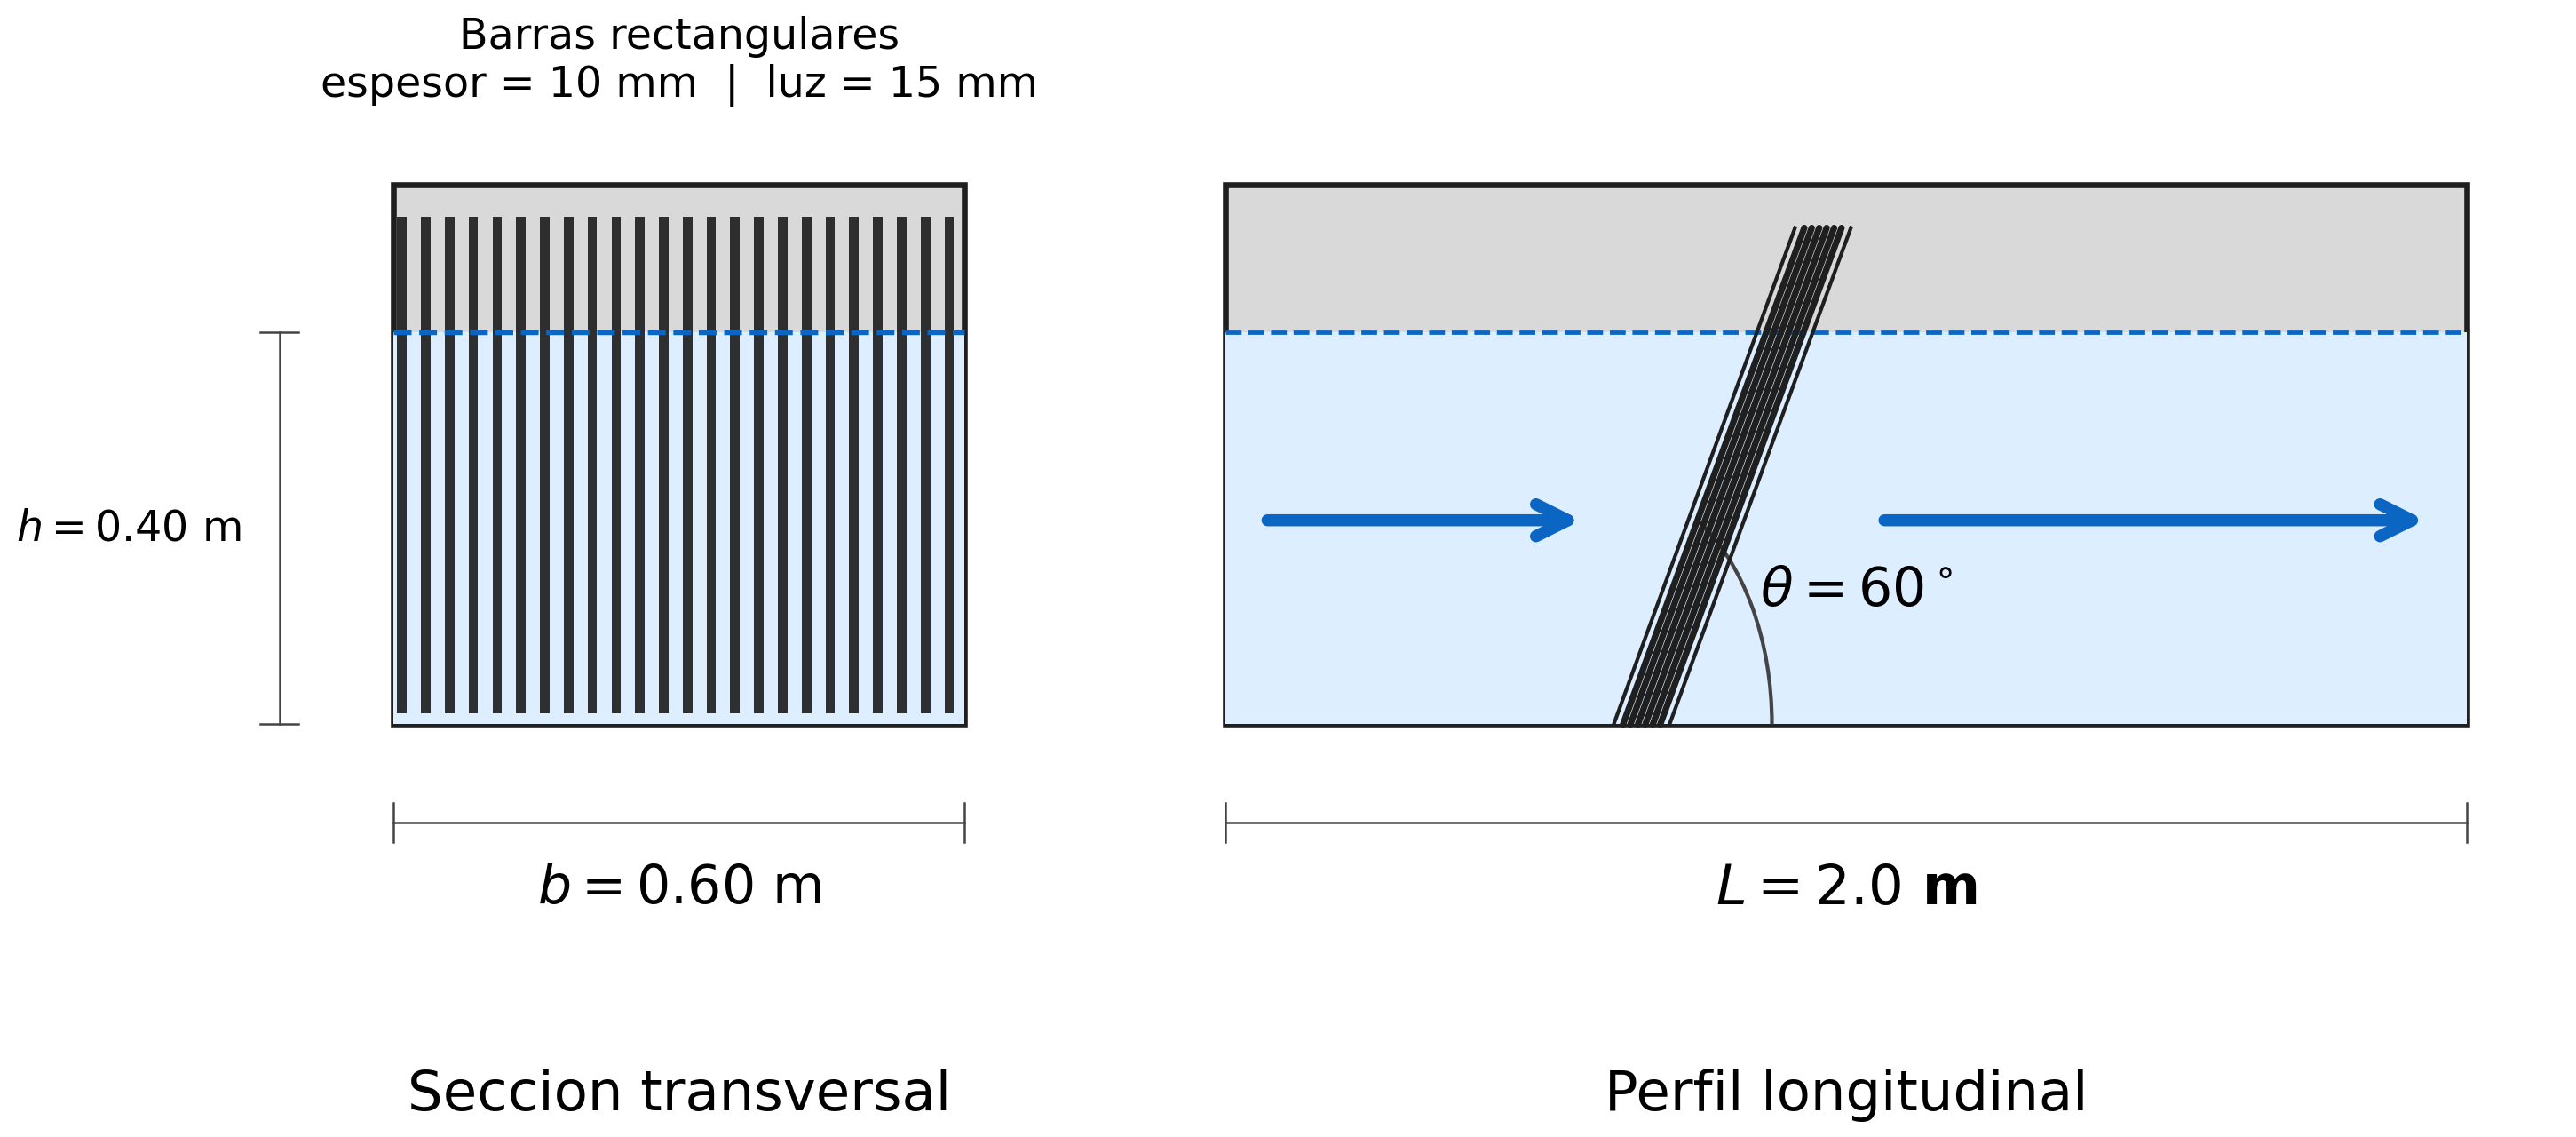
\includegraphics[width=0.9\textwidth]{figuras/rejillas_rejillas.png}
\caption{Esquema del canal de desbaste con rejillas (dimensiones en metros)}
\label{fig:rejillas}
\end{figure}





\textit{Nota sobre cantidades:} El presente dimensionamiento no estima la masa o volumen diario de residuos de cribado. Segun Metcalf y Eddy \cite{metcalf2014}, la produccion tipica de residuos de rejillas finas en aguas residuales municipales varia entre 0.005--0.02 m\textsuperscript{3}/1000 m\textsuperscript{3} de agua tratada. Para el caudal de diseno, esto representaria aproximadamente 0.02--0.09 m\textsuperscript{3}/d (total planta), sujeto a caracterizacion local.

Las dimensiones finales del canal con rejillas son: ancho 0.60 m, tirante 0.40 m y longitud 2.0 m. Se requieren dos unidades, una por cada linea de tratamiento.

\subsection{Desarenador de Flujo Horizontal}



El desarenador remueve part\'iculas minerales (arena, grava) con di\'ametro superior a 0.20~mm mediante sedimentaci\'on gravitacional. Seg\'un Metcalf y Eddy \cite{metcalf2014}, los par\'ametros de dise\~no son: velocidad horizontal 0.25--0.30~m/s (m\'aximo 0.30~m/s para evitar arrastre de sedimentos), tiempo de retenci\'on 30--60~s, y profundidad de flujo 0.75--2.0~m (OPS/CEPIS \cite{ops2005} permite valores menores en plantas peque\~nas).

La profundidad total del canal incluye: profundidad \'util de flujo (0.40~m), zona de almacenamiento de arena (0.25--0.30~m; se adopta 0.30~m), y bordo libre (0.30~m).

El dise\~no del desarenador se fundamenta en la teor\'ia de sedimentaci\'on discreta. Primero se calcula la velocidad de sedimentaci\'on de las part\'iculas objetivo mediante la Ley de Stokes:

\begin{equation}
v_s = \frac{g \cdot (S_s - 1) \cdot d^2}{18 \cdot \nu}
\end{equation}
\captionequation{Ley de Stokes - Velocidad de sedimentacion de particulas}

\textit{Donde:}
\begin{itemize}[noitemsep,leftmargin=2em]
    \item[$v_s$] = Velocidad de sedimentaci\'on (m/s)
    \item[$g$] = Aceleraci\'on de la gravedad (9.81 m/s²)
    \item[$S_s$] = Gravedad espec\'ifica de la arena (2.65)
    \item[$d$] = Di\'ametro de la part\'icula (0.00020 m)
    \item[$\nu$] = Viscosidad cinem\'atica del agua a 25.6°C ($8.3973e-07$ m²/s)
\end{itemize}

\begin{equation}
v_s = \frac{9.81 \times (2.65 - 1) \times (0.00020)^2}{18 \times 8.3973e-07} = 0.043 \text{ m/s}
\end{equation}

Con este valor de $v_s$ se determina la longitud te\'orica del desarenador mediante la ecuaci\'on de sedimentaci\'on tipo I:

\begin{equation}
L = \frac{H \cdot v_h}{v_s} = \frac{0.40 \times 0.30}{0.043} = 2.8 \text{ m}
\end{equation}

\textit{Donde:}
\begin{itemize}[noitemsep,leftmargin=2em]
    \item[$L$] = Longitud del desarenador (m)
    \item[$H$] = Profundidad \'util (0.40 m)
    \item[$v_h$] = Velocidad horizontal adoptada (0.30 m/s)
\end{itemize}

La longitud te\'orica resultante (2.8~m) es adecuada para el caudal de dise\~no y se adopta como longitud de dise\~no.

El ancho del canal se determina por la ecuaci\'on de continuidad:

\begin{equation}
B = \frac{Q}{v_h \cdot H} = \frac{0.00577}{0.30 \times 0.40} = 0.048 \text{ m}
\end{equation}

\textit{Donde:}
\begin{itemize}[noitemsep,leftmargin=2em]
    \item[$B$] = Ancho te\'orico del canal (m)
    \item[$Q$] = Caudal de dise\~no (0.00577 m³/s)
\end{itemize}

El ancho te\'orico resulta inferior al m\'inimo constructivo. Se adopta 0.60 m seg\'un OPS/CEPIS \cite{ops2005} y SENAGUA \cite{senagua2012}, que establecen 0.60 m como ancho m\'inimo para operaci\'on y mantenimiento.

Verificando la velocidad horizontal real con el ancho adoptado:

\begin{equation}
v_{real} = \frac{Q}{B \cdot H} = \frac{0.00577}{0.60 \times 0.40} = 0.024 \text{ m/s}
\end{equation}

El tiempo de retenci\'on real resulta:

\begin{equation}
t_r = \frac{L}{v_{real}} = \frac{3.0}{0.024} = 124.8 \text{ s}
\end{equation}

\subsubsection{Verificacion}

\textbf{Verificacion de Velocidad Critica de Resuspension}

Para garantizar que la arena sedimentada no sea resuspendida por el flujo, se verifica que la velocidad horizontal del dise\~no sea menor que la velocidad cr\'itica de resuspensi\'on, calculada mediante la f\'ormula de Camp-Shields:

\begin{equation}
v_c = \sqrt{\frac{8 \beta g (S_s - 1) d}{f}}
\end{equation}
\captionequation{Velocidad critica de resuspension - Camp-Shields}

\textit{Donde:}
\begin{itemize}[noitemsep,leftmargin=2em]
    \item[$v_c$] = Velocidad cr\'itica de resuspensi\'on (m/s)
    \item[$\beta$] = Factor de forma (0.05, rango 0.04--0.06)
    \item[$g$] = Aceleraci\'on de la gravedad (9.81 m/s²)
    \item[$S_s$] = Gravedad espec\'ifica de la arena (2.65)
    \item[$d$] = Di\'ametro de la part\'icula (0.00020 m)
    \item[$f$] = Factor de fricci\'on de Darcy-Weisbach (0.025, rango 0.02--0.03)
\end{itemize}

\begin{equation}
v_c = \sqrt{\frac{8 \times 0.05 \times 9.81 \times (2.65 - 1) \times 0.00020}{0.025}} = 0.228 \text{ m/s}
\end{equation}
\captionequation{Velocidad critica calculada}

\textbf{Verificacion para Caudal Maximo Horario}

Se verifica el comportamiento hidr\'aulico para el caudal m\'aximo horario, aplicando un factor de pico t\'ipico de 2.8 sobre el caudal medio:

\begin{equation}
Q_{max} = 2.8 \times Q_{medio} = 2.8 \times 5.8 = 16.0 \text{ L/s}
\end{equation}

A caudal m\'aximo, la velocidad horizontal resulta:

\begin{equation}
v_{h,max} = \frac{Q_{max}}{B \cdot H} = \frac{15.983/1000}{0.60 \times 0.40} = 0.067 \text{ m/s}
\end{equation}

El tiempo de retenci\'on a caudal m\'aximo:

\begin{equation}
t_{r,max} = \frac{L}{v_{h,max}} = \frac{3.0}{0.067} = 45.0 \text{ s}
\end{equation}

\textbf{Criterios de verificaci\'on de resuspensi\'on} (Camp-Shields, Metcalf y Eddy \cite{metcalf2014}):

La velocidad calculada $v_{h,max} = 0.067$~m/s se eval\'ua seg\'un (l\'imite: $v_c \times 90\% = 0.205$~m/s):

\begin{equation}
\text{Estado} = \begin{cases}
    \text{SEGURIDAD} & \text{si } v_{h,max} \leq 0.205 \text{ m/s} \quad \text{(no hay resuspensi\'on)} \\
    \text{RIESGO} & \text{si } v_{h,max} > 0.205 \text{ m/s} \quad \text{(arena resuspendida)}
\end{cases}
\end{equation}
\captionequation{Criterios de verificacion de resuspension}

Con la velocidad calculada $v_{h,max} = 0.067$~m/s, la unidad se clasifica como \textbf{SEGURIDAD}. En terminos de cumplimiento, la verificacion de resuspension \textbf{CUMPLE} porque es menor que el limite de resuspension con factor de seguridad (0.205~m/s), por lo que no se produce resuspension de la arena depositada.

\subsubsection{Resultados}

\begingroup
\small
\begin{longtable}{l p{9cm}}
\caption{Dimensiones del desarenador}\\
\toprule
Par\'ametro & Valor \\
\midrule
\endfirsthead
\caption[]{Dimensiones del desarenador (continuación)}\\
\toprule
Par\'ametro & Valor \\
\midrule
\endhead
\midrule
\multicolumn{2}{r}{\textit{Continúa en la siguiente página}} \\
\endfoot
\bottomrule
\endlastfoot
Longitud dise\~no & 3.0 m (m\'inimo constructivo SENAGUA) \\
Ancho & 0.60 m (m\'inimo constructivo) \\
Profundidad \'util & 0.40 m \\
Velocidad horizontal real & 0.024 m/s \\
Velocidad cr\'itica resuspensi\'on & 0.228 m/s (Camp-Shields) \\
Tiempo retenci\'on real & 124.8 s \\
\multicolumn{2}{p{\textwidth}}{\small\textit{$^a$Nota: El TRH de 125~s y velocidad de 0.024~m/s se deben al ancho m\'inimo constructivo de 0.60~m. }} \\
\end{longtable}
\endgroup

\textbf{Manejo de arena removida}

El desarenador retiene part\'iculas minerales, principalmente arena y grava fina, que se sedimentan en el fondo del canal por acci\'on gravitacional. Estas part\'iculas presentan di\'ametros superiores a 0.20~mm, con gravedad espec\'ifica de 2.65, correspondiendo a s\'olidos inorg\'anicos de alta densidad presentes en el agua residual. El canal incorpora una zona de almacenamiento de 0.30~m de altura, dimensionada espec\'ificamente para acumular la arena removida entre operaciones de limpieza. La frecuencia de limpieza recomendada es diaria o seg\'un la acumulaci\'on observada, manteniendo la arena acumulada por debajo del 50\% de la altura de almacenamiento designada para garantizar el funcionamiento \'optimo del sistema. La remoci\'on se realiza manualmente mediante palas y cubos desde la plataforma de operaci\'on, aunque puede implementarse un sistema de succi\'on o bombeo si el caudal y la producci\'on de arena lo justifican t\'ecnicamente.

\textbf{Disposici\'on final de la arena:}

La arena removida en el desarenador puede manejarse de diferentes formas seg\'un su composici\'on y la normativa local vigente. La opci\'on m\'as com\'un es el relleno sanitario, ya que la arena es material inorg\'anico inerte que puede disposicionarse en rellenos autorizados sin restricciones especiales. En caso de que la arena est\'e relativamente limpia, con bajo contenido de materia org\'anica adherida, existe la posibilidad de reuso condicionado para relleno y compactaci\'on en obras civiles previa caracterizaci\'on, mezcla con concreto para elementos no estructurales, o como complemento en sistemas de filtraci\'on gruesa previo lavado. Si se detecta alta carga org\'anica adherida a los granos de arena, evidenciada por olor f\'etido o color oscuro, se recomienda un lavado previo antes de la disposici\'on final para reducir el impacto ambiental.

\begin{figure}[H]
\centering

\includegraphics[width=\textwidth]{figuras/Esquema_Desarenador.png}
\caption{Esquema del desarenador de flujo horizontal con perfil longitudinal y corte transversal. Se muestran la entrada del afluente, la zona de flujo, el dep\'osito de arena y la salida . }
\label{fig:desarenador}
\end{figure}

\textit{Nota sobre cantidades:} El presente dimensionamiento no estima la masa o volumen diario de arena removida. Seg\'un Metcalf y Eddy \cite{metcalf2014}, la producci\'on t\'ipica de arena en aguas residuales municipales var\'ia entre 0.004--0.15 L/m\textsuperscript{3} de agua tratada, dependiendo de las caracter\'isticas del sistema de alcantarillado (red combinada vs. separada) y del suelo local. Para el caudal de dise\'no, esto representar\'ia aproximadamente 0.02--0.6 L/d (total planta), sujeto a caracterizaci\'on local.

\subsection{Reactor Anaerobio con Pantallas (ABR/RAP)}

\subsubsection{Dimensionamiento}

\textbf{Nomenclatura del reactor:} En la literatura técnica internacional, el reactor objeto de este manual se denomina ABR (\textit{Anaerobic Baffled Reactor}). En la literatura hispanohablante y en particular en los manuales de la OPS/OMS para saneamiento en países de desarrollo, se utiliza con frecuencia la sigla RAP (Reactor Anaerobio con Pantallas), que traduce literalmente el mismo concepto. Este documento adopta la denominación ABR como nombre principal del documento y del módulo de cálculo, por ser el término de uso universal en la bibliografía técnica de referencia. La sigla RAP se utiliza en paralelo en los títulos y encabezados del documento —de ahí la denominación compuesta "ABR / RAP"— con el fin de garantizar la trazabilidad con los manuales de la OPS/OMS que sirven de referencia complementaria en este proyecto.

\textbf{¿Qué es un Reactor Anaerobio con Pantallas (ABR / RAP)?}

El Reactor Anaerobio con Pantallas —ABR por sus siglas en inglés— es un sistema de tratamiento biológico anaerobio de aguas residuales que opera mediante flujo a través de una serie de compartimentos separados por pantallas o tabiques verticales (bafles). El agua residual entra por un extremo del reactor y recorre, en serie, cada uno de los compartimentos hasta llegar al extremo opuesto donde descarga el efluente tratado. En cada compartimento, el flujo sigue un patrón alternado de ascenso y descenso determinado por la posición y configuración de las pantallas.

El ABR fue desarrollado y descrito formalmente por McCarty y colaboradores en la Universidad de Stanford (Bachmann et al., 1985) como una evolución simplificada de los reactores anaerobios de lecho de lodos. Su gran ventaja conceptual sobre el reactor UASB (\textit{Upflow Anaerobic Sludge Blanket}) es la ausencia de un separador trifásico: la retención de la biomasa se logra por medios puramente hidráulicos y gravitacionales, aprovechando el hecho de que el flujo ascendente en cada compartimento es suficientemente lento como para mantener el manto de lodos en posición estable.

El ABR ocupa una posición intermedia entre el tanque séptico y el UASB en cuanto a complejidad constructiva y eficiencia de tratamiento. Es más eficiente que el tanque séptico porque el tratamiento ocurre en múltiples etapas en serie, cada una con su propia comunidad microbiana especializada. Es más simple que el UASB porque no requiere el separador trifásico, que es el componente más costoso y delicado de ese reactor. Esta combinación de buena eficiencia y simplicidad constructiva lo convierte en una opción especialmente adecuada para sistemas de saneamiento descentralizados, comunidades rurales y pequeñas cabeceras parroquiales en países de ingresos medios y bajos.

\textbf{Rol en el tren de tratamiento del proyecto:}

En el presente proyecto, el ABR se diseña como unidad de tratamiento primario anaerobio, situada aguas abajo del pretratamiento (cribado y desarenado) y aguas arriba de las unidades de tratamiento complementario o secundario. Su función principal es la remoción de materia orgánica en condiciones anaerobias, la estabilización parcial de los sólidos sedimentables y la acumulación y digestión \textit{in situ} de los lodos generados.

En la configuración típica del proyecto, el ABR reemplaza o complementa al tanque séptico convencional en situaciones donde se requiere un mayor nivel de remoción de DBO y DQO en la etapa anaerobia, con mayor control del proceso y sin la necesidad de un sistema mecánico de aireación. El efluente del ABR puede destinarse a un campo de infiltración, a un humedal de flujo subsuperficial, a un filtro anaerobio de flujo ascendente (FAFA) o, según el nivel de tratamiento requerido, a una etapa de tratamiento aerobio posterior (biofiltro, lodos activados, etc.).

\textbf{Principio de funcionamiento por compartimentos:}

El ABR es un reactor rectangular dividido internamente en una serie de compartimentos por medio de tabiques o pantallas verticales. Los tabiques no llegan completamente al fondo ni completamente a la superficie: dejan aberturas alternadas para forzar el recorrido del agua a través de toda la altura de cada compartimento.

En la configuración adoptada en este proyecto, los tabiques tienen una abertura en la parte inferior. El agua entra por el primer compartimento por el fondo, sube a través de él, desborda por encima del tabique intermedio o pasa por una abertura superior, desciende hasta el fondo del segundo compartimento, vuelve a subir, y así sucesivamente hasta el último compartimento. Este patrón de flujo ascendente-descendente garantiza que el agua atraviese toda la profundidad del manto de lodos en cada compartimento, maximizando el contacto entre el sustrato y la biomasa.

\textbf{Retención de biomasa sin separador trifásico:}

La clave del funcionamiento del ABR es la velocidad ascensional relativamente baja en el interior de cada compartimento. El manto de lodos anaerobio se mantiene en posición porque la velocidad ascendente del flujo no es suficiente para arrastrar los gránulos o flóculos de lodo hacia el compartimento siguiente. Esta retención es fundamentalmente diferente a la del UASB, donde se requiere un separador trifásico para capturar los sólidos que el flujo ascendente tiende a arrastrar hacia la superficie: en el ABR, la propia geometría del sistema asegura que la velocidad ascensional se mantenga por debajo del umbral de arrastre del lodo, sin necesidad de separadores mecánicos adicionales.

La consecuencia práctica es que en el ABR cada compartimento acumula su propia población microbiana, y esa población se adapta progresivamente a la calidad del agua que recibe: el primer compartimento, que recibe el agua cruda más concentrada, contiene predominantemente bacterias hidrolíticas y acidogénicas; los compartimentos intermedios tienen una mezcla de acidogénicos y acetogénicos; y el último compartimento, que recibe un agua ya considerablemente tratada, tiene condiciones más propicias para los metanogénicos. Esta separación funcional a lo largo del reactor es uno de los factores que explican la robustez del ABR frente a variaciones de carga.

\textbf{Mecanismos principales de remoción:}

Los mecanismos de remoción en el ABR son los propios del tratamiento anaerobio en cuatro etapas clásicas:

\textit{Hidrólisis:} Las moléculas orgánicas complejas (proteínas, grasas, hidratos de carbono) son fraccionadas en monómeros y dímeros por enzimas extracelulares producidas por las bacterias hidrolíticas. Esta etapa es generalmente la limitante del proceso para residuales con alta concentración de sólidos particulados.

\textit{Acidogénesis:} Los productos de la hidrólisis son fermentados por bacterias acidogénicas a ácidos grasos volátiles (AGV), alcoholes, dióxido de carbono e hidrógeno. Esta etapa es generalmente rápida en comparación con la hidrólisis y con la metanogénesis.

\textit{Acetogénesis:} Los ácidos grasos volátiles de cadena corta (propionato, butirato) son convertidos a acetato, CO$_2$ e H$_2$ por bacterias acetogénicas. Esta etapa es termodinámicamente desfavorable a concentraciones altas de H$_2$ y solo ocurre de forma eficiente cuando el hidrógeno es consumido rápidamente por organismos hidrogenotróficos (sintrofía obligada).

\textit{Metanogénesis:} El acetato y el H$_2$/CO$_2$ son convertidos a metano y CO$_2$ por las arqueas metanogénicas. Esta etapa es la más sensible a variaciones de pH y temperatura, y la que limita la tasa global del proceso cuando el sistema está correctamente operado.

Adicionalmente, en el ABR ocurre sedimentación de sólidos suspendidos por efecto de la reducción de velocidad dentro de cada compartimento: los sólidos gruesos que no se degradan rápidamente sedimentan en el fondo del primer compartimento o de los primeros compartimentos, donde se acumulan y se digieren lentamente. Esta función es análoga a la del tanque séptico, pero con la ventaja de que el tratamiento biológico activo ocurre en paralelo y de forma mucho más eficiente.

\textbf{Criterios de diseño adoptados por el proyecto:}

Los siguientes parámetros han sido seleccionados como criterios de diseño para el reactor ABR, basados en la bibliografía técnica y adaptados a las condiciones del proyecto:

\begin{table}[H]
\centering
\caption{Parámetros seleccionados para el diseño ABR / RAP}
\begin{tabular}{p{6cm}cc}
\toprule
\textbf{Parámetro} & \textbf{Valor adoptado} & \textbf{Rango recomendado} \\
\midrule
Tiempo de retención hidráulico (TRH) & 24 h & 24--72 h \\
Número de compartimentos ($n$) & 4 & 2--8 (recomendado: 4--6) \\
Velocidad ascensional de diseño ($v_{up}$) & 1.0 m/h & 0,2--1,5 m/h \\
Profundidad útil del líquido ($H$) & 2.0 m & 1,5--3,0 m \\
Zona de acumulación de lodos & 0.30 m & 0,2--0,5 m \\
Bordo libre & 0.30 m & $\geq$ 0,30 m \\
\bottomrule
\end{tabular}
\end{table}

\textit{Nota: Estos valores son criterios adoptados por el proyecto basados en Barber \& Stuckey (1999), Foxon et al. (2004) y OPS/OMS (2005). No son límites normativos impuestos por la TULSMA ni por normas ecuatorianas específicas para reactores anaerobios.}

\textbf{Ecuaciones de dimensionamiento:}

El dimensionamiento del ABR se fundamenta en el criterio del tiempo de retención hidráulico (TRH) y en la verificación de la velocidad ascensional. Las ecuaciones fundamentales son las siguientes:

\textbf{[Ecuación 1] Volumen total del reactor:}

\begin{equation}
V_{total} = Q_{medio} \times TRH
\end{equation}

\textit{Donde:}
\begin{itemize}[noitemsep,leftmargin=2em]
    \item[$V_{total}$] = Volumen total del reactor (m³)
    \item[$Q_{medio}$] = Caudal medio diario de diseño (498.5 m³/d = 20.77 m³/h)
    \item[$TRH$] = Tiempo de retención hidráulico adoptado (24 h = 1.00 d)
\end{itemize}

Sustituyendo los valores del proyecto:

\begin{equation}
V_{total} = 498.5 \times 1.000 = 498.5 \text{ m}^3
\end{equation}

\textbf{[Ecuación 2] Volumen por compartimento:}

\begin{equation}
V_{comp} = \frac{V_{total}}{n} = \frac{498.5}{4} = 124.63 \text{ m}^3
\end{equation}

\textbf{[Ecuación 3] Área de sección transversal por velocidad ascensional:}

La velocidad ascensional es el parámetro crítico que controla la retención de la biomasa en el reactor. Para que el ABR funcione correctamente, la velocidad ascensional debe ser inferior a la velocidad de sedimentación de los flóculos de lodo.

\begin{equation}
A_{transversal} = \frac{Q_{medio}}{v_{up, dise\tilde{n}o}} = \frac{20.77}{1.0} = 20.77 \text{ m}^2
\end{equation}

\textbf{[Ecuación 4] Dimensiones del reactor:}

A partir del área de sección transversal y la profundidad útil adoptada, se obtienen las dimensiones geométricas:

\begin{equation}
W = \frac{A_{transversal}}{H} = \frac{20.77}{2.0} = 10.39 \text{ m} \quad \text{(ancho)}
\end{equation}

\begin{equation}
L_{comp} = \frac{V_{comp}}{W \times H} = \frac{124.63}{10.39 \times 2.0} = 6.00 \text{ m} \quad \text{(largo por compartimento)}
\end{equation}

\begin{equation}
L_{total} = n \times L_{comp} = 4 \times 6.00 = 24.00 \text{ m} \quad \text{(largo total)}
\end{equation}

La profundidad total de construcción incluye la profundidad útil del líquido, la zona de acumulación de lodos y el bordo libre:

\begin{equation}
H_{total} = H + H_{lodos} + H_{bordo} = 2.0 + 0.30 + 0.30 = 2.60 \text{ m}
\end{equation}

\textbf{[Ecuación 5] Altura de abertura en los bafles (slot inferior):}

Cada pantalla o bafle interno no ocupa toda la altura del compartimento: deja una abertura en su parte inferior (slot) por la que el flujo debe pasar antes de ascender en el compartimento siguiente. La altura de este slot es un parámetro de diseño que determina la velocidad puntual del flujo en la transición entre compartimentos. Según OPS/OMS (2005) y Foxon et al. (2004), esta abertura se define como una fracción de la profundidad útil, típicamente entre el 15\,\% y el 25\,\% de $H$. Adoptando el valor central de la bibliografía ($f_{slot} = 0.20$):

\begin{equation}
h_{slot} = f_{slot} \times H = 0.20 \times 2.0 = 0.40 \text{ m}
\end{equation}

\textbf{[Ecuación 6] Velocidad en la abertura de los bafles:}

La velocidad del flujo al atravesar la abertura inferior de cada bafle (\textit{slot velocity}) es significativamente mayor que la velocidad ascensional media del compartimento, porque el área de paso queda reducida a $W \times h_{slot}$. Este parámetro es crítico: un valor excesivo genera turbulencia local en el fondo del compartimento siguiente, resuspende los lodos sedimentados y puede provocar su arrastre hacia el efluente. La bibliografía recomienda mantener esta velocidad por debajo de 1.0~m/h a caudal medio:

\begin{equation}
v_{slot} = \frac{Q_{medio}}{W \times h_{slot}} = \frac{20.770}{10.39 \times 0.40} = 5.00 \text{ m/h}
\end{equation}

\textbf{Limitaciones del método actual:}

El presente dimensionamiento cubre el cálculo del volumen total, número y tamaño de compartimentos, geometría del reactor, verificaciones hidráulicas y parámetros de carga. No cubre, en esta versión del cálculo: el modelado de la eficiencia de remoción de DBO en función del TRH (que requeriría un modelo cinético calibrado), el cálculo de la producción de biogás, el diseño del sistema de ventilación del biogás, el balance detallado de lodos en estado estacionario, ni el dimensionamiento de tuberías de entrada, salida y extracción de lodos.

\subsubsection{Verificación}

La subsección de verificación evalúa de forma sistemática si el reactor dimensionado satisface los criterios hidráulicos y geométricos de la bibliografía de referencia. Para cada verificación se describe primero el fenómeno físico que la motiva, después se desarrolla el cálculo con los valores del proyecto y, finalmente, se emite el juicio de cumplimiento. Se distinguen verificaciones \textbf{obligatorias} ---cuyo incumplimiento invalida el diseño--- de \textbf{complementarias} ---que orientan sobre la calidad del diseño sin invalidarlo--- y de \textbf{parámetros informativos} ---que no tienen criterio de cumplimiento en este nivel de diseño---.

\textbf{Verificaciones obligatorias:}

\textbf{[V-1] Rango bibliográfico de la velocidad ascensional de diseño}

El primer parámetro que debe justificarse es la propia elección de la velocidad ascensional de diseño $v_{up,dise\tilde{n}o} = 1.0$~m/h. Este valor no es un resultado del cálculo sino una decisión del proyectista: determina el área transversal del reactor (Ecuación~3) y, a través de ella, todas las demás dimensiones geométricas. Su validez depende de que se encuentre dentro del rango operativo aceptable reportado en la bibliografía técnica.

Las razones de este límite son físicas: velocidades demasiado altas generan shear suficiente para arrastrar los flóculos de lodo anaerobio hacia el efluente, empobreciendo progresivamente la biomasa activa del reactor; velocidades demasiado bajas producen reactores sobredimensionados sin mejora proporcional en la eficiencia biológica, pues el limitante del proceso pasa a ser la cinética de la metanogénesis y no el tiempo de contacto. Según Foxon et al. (2004) y Barber \& Stuckey (1999), el rango operativo aceptable para aguas residuales domésticas a temperatura ambiente es:

\begin{equation}
0.2 \text{ m/h} \leq v_{up,dise\tilde{n}o} \leq 1.5 \text{ m/h}
\end{equation}

El valor adoptado en este proyecto es $v_{up,dise\tilde{n}o} = 1.0$~m/h.

\textit{Nota importante sobre la verificación de la velocidad a caudal medio:} la velocidad ascensional calculada a caudal medio ($v_{up,calc} = Q_{medio} / (W \times H)$) coincide por construcción con $v_{up,dise\tilde{n}o}$, puesto que el ancho $W$ se obtuvo directamente como $W = Q_{medio} / (v_{up,dise\tilde{n}o} \times H)$. No existe por tanto una verificación numérica independiente a caudal medio: la verificación real y crítica de la velocidad ascensional es la del caudal pico (V-2), que sí puede superar el límite admisible.

Estado V-1: \textbf{CUMPLE} ($0.2 \leq 1.0 \leq 1.5$~m/h)

\textbf{[V-2] Velocidad ascensional a caudal máximo horario}

Esta es la verificación hidráulica más crítica del diseño. Durante los picos de consumo ---generalmente en las mañanas y mediodías en sistemas domésticos--- el caudal supera al medio en un factor de pico $f_p$. Si en esas condiciones la velocidad ascensional rebasa el umbral de arrastre, la biomasa abandona el reactor con el efluente y el rendimiento de depuración se deteriora progresivamente. A diferencia del UASB, el ABR carece de separador trifásico que retenga los sólidos en esas condiciones: la única salvaguarda es que la geometría garantice una velocidad admisible incluso en pico.

El caudal pico horario se obtiene aplicando el factor de pico al caudal medio de diseño:

\begin{equation}
Q_{max} = f_p \times Q_{medio} = 2.8 \times 20.770 = 57.540 \text{ m}^3\text{/h}
\end{equation}

Con este caudal, la velocidad ascensional en pico resulta:

\begin{equation}
v_{up,max} = \frac{Q_{max}}{W \times H} = \frac{57.540}{10.39 \times 2.0} = 2.77 \text{ m/h}
\end{equation}

El límite bibliográfico para caudal pico, según Barber \& Stuckey (1999), es de 2.0~m/h. Por encima de este umbral se ha observado exportación significativa de sólidos hacia el efluente en reactores piloto y a escala real.

Criterio: $v_{up,max} \leq 2.0$~m/h

Estado V-2: \textbf{NO CUMPLE} (2.77~m/h $>$ 2.0~m/h)

\textbf{[V-3] Verificación del tiempo de retención hidráulico por geometría}

El TRH de diseño fija el volumen total del reactor (Ecuación~1). Sin embargo, las dimensiones finales resultan de una cadena de operaciones aritméticas ---división por área, multiplicación por número de compartimentos--- que en la práctica pueden ajustarse a valores constructivos enteros. Esta verificación confirma que el volumen efectivo de la geometría adoptada reproduce, o supera, el TRH de diseño. Si el TRH calculado resultara inferior al de diseño, significaría que las dimensiones son insuficientes y que el tiempo de contacto nominal no se alcanzaría en la práctica.

\begin{equation}
TRH_{calc} = \frac{L_{total} \times W \times H_{util}}{Q_{medio}} \times 24 = \frac{24.00 \times 10.39 \times 2.0}{498.5} \times 24 = 24.0 \text{ h}
\end{equation}

Criterio: $TRH_{calc} \geq 24$~h

Estado V-3: \textbf{CUMPLE} (24.0~h $\geq$ 24~h)

\textbf{[V-4] Largo mínimo de compartimento}

El largo de cada compartimento ($L_{comp}$) debe satisfacer dos criterios independientes que responden a razones diferentes. El criterio constructivo establece un mínimo absoluto de 1.0~m: por debajo de esta dimensión el compartimento es impracticable desde el punto de vista de la ejecución de obra, la inspección y la extracción de lodos. El criterio hidráulico-bibliográfico, según OPS/OMS (2005), establece que $L_{comp} \geq H_{util}$: esta condición garantiza que el recorrido horizontal del flujo sea suficiente para que los sólidos gruesos no degradados sedimenten antes de alcanzar el bafle siguiente, evitando cortocircuitos hidráulicos. Ambos criterios deben cumplirse simultáneamente, por lo que el largo mínimo efectivo es el mayor de los dos valores:

\begin{equation}
L_{comp,min} = \max\!\left(H_{util},\; 1.0\right) = \max\!\left(2.0,\; 1.0\right) = 2.0 \text{ m}
\end{equation}

Valor calculado: $L_{comp} = 6.00$~m

Estado V-4: \textbf{CUMPLE} ($L_{comp} = 6.00$~m $\geq$ 2.0~m)

\textbf{[V-5] Velocidad en la abertura inferior de los bafles (\textit{slot velocity})}

Cada pantalla interna del ABR deja una abertura en su parte inferior (denominada \textit{slot} en la bibliografía anglosajona) a través de la cual el flujo pasa de un compartimento al siguiente antes de ascender. Dado que el área de esta abertura ($W \times h_{slot}$) es sustancialmente menor que el área transversal total del compartimento ($W \times H$), la velocidad puntual del flujo en el slot es notablemente mayor que la velocidad ascensional media.

Esta aceleración local tiene dos efectos negativos cuando supera el umbral admisible: primero, genera turbulencia en el fondo del compartimento receptor, resuspendiendo los flóculos de lodo ya sedimentados; segundo, puede crear zonas de mezcla intensa que cortocircuitan la separación funcional entre compartimentos, que es uno de los fundamentos del buen rendimiento del ABR. OPS/OMS (2005) y Foxon et al. (2004) recomiendan definir la abertura como el 20\,\% de la profundidad útil ($f_{slot} = 0.20$) y mantener la velocidad en el slot por debajo de 1.0~m/h a caudal medio:

\begin{equation}
h_{slot} = f_{slot} \times H_{util} = 0.20 \times 2.0 = 0.40 \text{ m}
\end{equation}

La velocidad en la abertura a caudal medio resulta:

\begin{equation}
v_{slot} = \frac{Q_{medio}}{W \times h_{slot}} = \frac{20.770}{10.39 \times 0.40} = 5.00 \text{ m/h}
\end{equation}

A modo informativo, a caudal máximo:

\begin{equation}
v_{slot,max} = \frac{Q_{max}}{W \times h_{slot}} = \frac{57.540}{10.39 \times 0.40} = 13.85 \text{ m/h}
\end{equation}

Criterio: $v_{slot} \leq 1.0$~m/h (caudal medio)

Estado V-5: \textbf{NO CUMPLE} (5.00~m/h $>$ 1.0~m/h)

\textbf{[V-6] Relación profundidad útil / ancho del reactor ($H/W$)}

La relación $H/W$ describe la forma de la sección transversal de cada compartimento. Su importancia es reconocida en la bibliografía reciente (Sinha et al., 2009): valores extremos en cualquier sentido comprometen la uniformidad del flujo vertical ascendente. Un reactor excesivamente ancho en relación con su profundidad ($H/W < 0.5$) tiende a tener distribución no uniforme del flujo en el plano transversal, con zonas muertas en los extremos laterales donde la velocidad ascensional es insuficiente para mantener el manto de lodos en suspensión activa. Por el contrario, un reactor excesivamente estrecho ($H/W > 2.0$) dificulta la distribución uniforme del afluente en el ancho y puede crear flujos preferenciales en la zona central que reducen el contacto efectivo entre el sustrato y la biomasa. El rango recomendado es:

\begin{equation}
0.5 \leq \frac{H_{util}}{W} \leq 2.0
\end{equation}

El valor calculado para este diseño es:

\begin{equation}
\frac{H_{util}}{W} = \frac{2.0}{10.39} = 0.19
\end{equation}

Estado V-6: \textbf{NO CUMPLE} ($0.5 \leq 0.19 \leq 2.0$)

\textbf{Verificaciones complementarias:}

\textbf{[V-7] Relación largo / ancho del compartimento ($L_{comp} / W$)}

La relación $L_{comp} / W$ describe la esbeltez en planta de cada compartimento. Compartimentos muy alargados ($L_{comp} / W > 2.0$) pueden presentar distribución no uniforme del afluente a lo largo del ancho; compartimentos muy cuadrados o anchos ($L_{comp} / W < 0.5$) tienden hacia un comportamiento de mezcla completa en el plano horizontal, reduciendo la eficiencia de la separación en serie entre compartimentos. El rango orientativo recomendado por la OPS/OMS (2005) es:

\begin{equation}
0.5 \leq \frac{L_{comp}}{W} \leq 2.0
\end{equation}

Valor calculado: $L_{comp} / W = 6.00 / 10.39 = 0.58$

Estado V-7: \textbf{DENTRO RANGO} (verificación complementaria)

\textbf{[V-8] Número mínimo de compartimentos}

El número de compartimentos determina el grado de separación funcional entre las fases del proceso anaerobio. Con un solo compartimento el ABR no tiene ventaja sobre un digestor de mezcla completa. A partir de cuatro compartimentos se logra una separación razonablemente clara entre las comunidades hidrolítico-acidogénicas (primer y segundo compartimento) y las metanogénicas (últimos compartimentos). La OPS/OMS (2005) establece un mínimo de 3 compartimentos para aplicaciones de saneamiento doméstico descentralizado:

\begin{equation}
n \geq 3
\end{equation}

Valor adoptado: $n = 4$

Estado V-8: \textbf{CUMPLE}

\textbf{Parámetros informativos:}

\textbf{[V-9] Carga orgánica volumétrica (COV)}

La carga orgánica volumétrica expresa la cantidad de materia orgánica que ingresa por unidad de volumen y por día. Es el parámetro de referencia más utilizado en la bibliografía de reactores anaerobios para comparar diseños y evaluar si el reactor opera en un régimen compatible con el mantenimiento de una biomasa estable. No constituye un criterio obligatorio en este diseño, pero permite situar el proyecto en el contexto de experiencias reportadas.

La DBO se expresa en mg/L, unidad equivalente a g/m³; dividirla entre 1\,000 convierte g a kg. La expresión completa con sus unidades explícitas es:

\begin{equation}
COV = \frac{Q_{medio} \,[\text{m}^3/\text{d}] \times DBO_{entrada} \,[\text{g/m}^3] \,/\, 1\,000}{V_{total} \,[\text{m}^3]} = \frac{498.5 \times 231 / 1\,000}{498.5} = 0.23 \text{ kg\,DBO/(m}^3\!\cdot\!\text{d)}
\end{equation}

Rango bibliográfico para ABR doméstico a temperatura ambiente: 0.5--5.0~kg\,DBO/(m³·d) (Barber \& Stuckey, 1999; OPS/OMS, 2005).

\textbf{[V-10] Estimación de la producción de lodos y frecuencia de purga}

La zona de acumulación de lodos reservada en el dimensionamiento ($H_{lodos} = 0.30$~m) debe ser coherente con la tasa real de producción de biomasa anaerobia en el reactor. Sin esta comprobación, el espacio reservado para lodos es solo un criterio empírico desconectado de las condiciones reales del proyecto. La OPS/OMS (2005, Capítulo~6) proporciona la siguiente expresión para una estimación de orden de magnitud:

\begin{equation}
P_{lodos} = Y_{obs} \times DBO_{rem}
\end{equation}

Donde $Y_{obs} \approx 0.10$~kg\,SSV/kg\,DBO\,removida es el rendimiento observado en digestión anaerobia mesofílica de aguas residuales domésticas (Rittmann \& McCarty, 2001), y $DBO_{rem}$ es la DBO removida diariamente. Adoptando la eficiencia de referencia bibliográfica del 75\,\%:

\begin{equation}
DBO_{rem} = \eta_{ref} \times DBO_{entrada} \times \frac{Q_{medio}}{1\,000} = 0.75 \times 231 \times \frac{498.5}{1\,000} = 86.35 \text{ kg\,DBO/d}
\end{equation}

\begin{equation}
P_{lodos} = 0.10 \times 86.35 = 8.63 \text{ kg\,SSV/d}
\end{equation}

Adoptando una densidad de lodos húmedos anaerobios espesados de $\rho = 1\,040$~kg/m³, el volumen acumulado anualmente es:

\begin{equation}
V_{lodos,año} = \frac{P_{lodos} \times 365}{\rho} = \frac{8.63 \times 365}{1\,040} = 3.03 \text{ m}^3\text{/año}
\end{equation}

El volumen disponible en la zona de lodos del reactor es:

\begin{equation}
V_{zona\,lodos} = L_{total} \times W \times H_{lodos} = 24.00 \times 10.39 \times 0.30 = 74.81 \text{ m}^3
\end{equation}

Esto implica una frecuencia indicativa de purga de lodos de aproximadamente \textbf{237 meses}, asumiendo extracción cuando la zona de acumulación alcanza el 80\,\% de su capacidad. Este valor es una estimación de orden de magnitud y deberá ajustarse en la puesta en marcha del sistema en función de las mediciones reales de producción de lodos.

\textbf{Resumen de verificaciones:}

\begin{table}[H]
\centering
\caption{Resumen de verificaciones del reactor ABR / RAP}
\begin{tabular}{llp{5.5cm}}
\toprule
\textbf{Verificación} & \textbf{Estado} & \textbf{Valor calculado vs. criterio} \\
\midrule
V-1 Rango v\_up diseño & \checkmark & 1.0 m/h $\in$ [0.2--1.5] m/h \\
V-2 v\_up caudal máximo & \texttimes & 2.77 m/h $\leq$ 2.0 m/h \\
V-3 TRH verificado & \checkmark & 24.0 h $\geq$ 24 h \\
V-4 Largo mínimo compartimento & \checkmark & L\_comp = 6.00 m $\geq$ 2.0 m \\
V-5 Velocidad abertura bafle & \texttimes & 5.00 m/h $\leq$ 1.0 m/h \\
V-6 Relación H/W & \texttimes & 0.19 $\in$ [0.5--2.0] \\
\bottomrule
\end{tabular}
\end{table}

\textbf{ATENCIÓN:} las siguientes verificaciones NO cumplen y requieren revisión del diseño: V-2 v\_up caudal máximo, V-5 Velocidad abertura bafle, V-6 Relación H/W.

\textit{Notas: (a) El proyecto NO calcula la eficiencia de remoción de DBO a partir de parámetros operacionales. Las eficiencias del 70--95\,\% reportadas en la bibliografía para ABR con TRH de 24~h son referencias y no predicciones garantizadas. (b) La estimación de producción de lodos (V-10) adopta una eficiencia de referencia del 75\,\%; el valor real dependerá de las condiciones de operación.}

\subsubsection{Resultados}

\begin{figure}[H]
\centering

\includegraphics[width=0.95\textwidth]{figuras/Esquema_ABR.png}
\caption{Esquema del Reactor Anaerobio con Pantallas (ABR / RAP) -- vista longitudinal}
\label{fig:esquema_abr}
\end{figure}

El dimensionamiento del Reactor Anaerobio con Pantallas (ABR / RAP) ha producido las siguientes dimensiones y parámetros de operación:

El esquema muestra la configuración típica del ABR con flujo en zigzag (\textit{up-flow} y \textit{down-flow}) a través de los compartimentos, las pantallas internas (\textit{baffles}) que dirigen el flujo, las zonas de lodos, líquida y biogás, así como los puntos de entrada, salida y ventilación.

\begin{longtable}{p{6cm}p{3cm}p{5cm}}
\caption{Resultados del dimensionamiento ABR / RAP} \\
\toprule
\textbf{Parámetro} & \textbf{Valor} & \textbf{Observación} \\
\midrule
\endfirsthead
\multicolumn{3}{c}{
    {\bfseries \tablename\ \thetable{} -- continuación de la página anterior}
} \\
\toprule
\textbf{Parámetro} & \textbf{Valor} & \textbf{Observación} \\
\midrule
\endhead
\midrule
\multicolumn{3}{r}{Continúa en la siguiente página...} \\
\endfoot
\bottomrule
\endlastfoot

\multicolumn{3}{l}{\textit{Parámetros de entrada:}} \\
Caudal medio ($Q_{medio}$) & 498.5 m³/d & Caudal por línea de tratamiento \\
Caudal máximo ($Q_{max}$) & 1380.9 m³/d & Factor pico: 2.8 \\
DBO afluente & 231 mg/L & Caracterización afluente \\
\midrule

\multicolumn{3}{l}{\textit{Criterios de diseño adoptados:}} \\
Tiempo retención hidráulico (TRH) & 24 h & Criterio del proyecto \\
Número de compartimentos ($n$) & 4 & 4--8 recomendado \\
Velocidad ascensional diseño & 1.0 m/h & $\leq$ 2.0 m/h límite pico \\
Profundidad útil ($H$) & 2.0 m & 1.5--3.0 m rango \\
\midrule

\multicolumn{3}{l}{\textit{Dimensiones geométricas:}} \\
Volumen total ($V_{total}$) & 498.5 m³ & Calculado por TRH \\
Volumen por compartimento & 124.63 m³ & Distribución uniforme \\
Área sección transversal & 20.77 m² & Por velocidad ascensional \\
Ancho del reactor ($W$) & 10.39 m & Geometría transversal \\
Largo por compartimento & 6.00 m & $L_{comp} \geq H$ verificado \\
Largo total ($L_{total}$) & 24.00 m & $n \times L_{comp}$ \\
Profundidad total construcción & 2.60 m & $H + H_{lodos} + H_{bordo}$ \\
Área en planta total & 249.26 m² & $L_{total} \times W$ \\
\midrule

\multicolumn{3}{l}{\textit{Parámetros hidráulicos:}} \\
Velocidad ascensional (caudal medio) & 1.00 m/h & CUMPLE \\
Velocidad ascensional (caudal máximo) & 2.77 m/h & NO CUMPLE \\
TRH calculado & 24.0 h & CUMPLE \\
Carga hidráulica superficial (CHS) & 2.00 m/d & Parámetro informativo \\
\midrule

\multicolumn{3}{l}{\textit{Parámetros de proceso (informativos):}} \\
Carga orgánica volumétrica (COV) & 0.23 kg/m³·d & Rango ref: 0.5--5.0 \\
\midrule

\multicolumn{3}{l}{\textit{Estado de verificaciones:}} \\
Verificación velocidad (medio) & CUMPLE & Criterio: $\leq$ 1.0 m/h \\
Verificación velocidad (máx) & NO CUMPLE & Criterio: $\leq$ 2.0 m/h \\
Verificación TRH & CUMPLE & Criterio: $\geq$ 24 h \\
Verificación largo comp. & CUMPLE & Criterio: $L_{comp} \geq H$ \\
\bottomrule
\multicolumn{3}{l}{\textbf{Estado general del diseño:} \textbf{REQUIERE REVISIÓN}} \\
\end{longtable}

\textbf{Notas sobre los resultados:}

El reactor ABR / RAP dimensionado consta de 4 compartimentos idénticos con una geometría rectangular de 24.00~m de largo total, 10.39~m de ancho y 2.60~m de profundidad total de construcción. La profundidad útil del líquido es de 2.0~m, con una zona adicional de 0.30~m reservada para acumulación de lodos y 0.30~m de bordo libre.

El diseño opera con una velocidad ascensional de 1.00~m/h a caudal medio, valor que se eleva hasta 2.77~m/h durante los picos de caudal. La velocidad a caudal medio cumple con el límite operativo, pero la velocidad de pico supera el umbral bibliográfico admisible (2.0~m/h), lo que indica que el reactor puede experimentar arrastre de biomasa en condiciones de caudal máximo y debe ser revisado.

El tiempo de retención hidráulico de 24.0~h (1.00~días) proporciona el tiempo de contacto necesario entre el agua residual y la biomasa anaerobia para la degradación de la materia orgánica. Este valor se encuentra dentro del rango recomendado de 24--72 horas para reactores ABR tratando aguas residuales domésticas.

\textbf{Alcance y limitaciones declaradas:}

Este dimensionamiento cubre el volumen del reactor, la geometría básica y las verificaciones hidráulicas fundamentales. No incluye: (a) predicción de la eficiencia de remoción de DBO o DQO mediante modelos cinéticos; (b) cálculo de la producción de biogás ni dimensionamiento del sistema de ventilación; (c) balance detallado de producción de lodos y frecuencia de extracción; (d) diseño de las pantallas internas (altura, espesor, configuración de aberturas); (e) dimensionamiento de tuberías de entrada, salida y extracción de lodos. Estos elementos constituyen extensiones futuras del diseño que deben desarrollarse según las condiciones específicas del proyecto.

\subsection{Biofiltro Biológico Aireado (BAF)}

\subsubsection{Dimensionamiento}

El Biofiltro Biológico Aireado (BAF, por sus siglas en inglés \textit{Biological Aerated Filter}) es un reactor biológico de biopelícula que opera con el lecho de relleno completamente sumergido y con suministro forzado de oxígeno mediante difusores de burbuja fina instalados en la base del reactor. Esta configuración lo distingue fundamentalmente del filtro percolador tradicional, en el que el agua gotea por gravedad sobre un relleno expuesto al aire ambiente. En el BAF el control de la aireación es activo, lo que permite mantener condiciones plenamente aerobias en toda la altura del lecho con independencia de la carga aplicada.

La característica más relevante del BAF desde el punto de vista del tren de tratamiento es su doble función: actúa simultáneamente como reactor biológico y como filtro físico. Los microorganismos adheridos al relleno degradan la materia orgánica disuelta, mientras que el propio lecho retiene los sólidos suspendidos y la biomasa que eventualmente se desprende del biofilm. El resultado es un efluente clarificado que puede enviarse directamente a desinfección sin necesidad de sedimentador secundario, lo que reduce la huella de planta entre un 30\,\% y un 50\,\% respecto a los sistemas convencionales de lodos activados.

En el presente proyecto el BAF ocupa la posición de tratamiento secundario aerobio aguas abajo del reactor UASB, cuyo efluente contiene típicamente entre 80 y 150\,mg/L de DBO y sólidos suspendidos de tamaño medio. Para el dimensionamiento se adopta una concentración de DBO a la entrada del BAF de $S_0 = 58$\,mg/L, valor conservador representativo del efluente UASB para este tipo de sistema.

\subsubsection*{Principio de Funcionamiento y Configuración}

El BAF opera sobre la base de una biopelícula aerobia estable adherida a un medio de relleno plástico modular de alta superficie específica ($S_{\text{esp}} = 250$\,m²/m³). El agua residual entra por la parte inferior del reactor y asciende a través del lecho en configuración \textit{up-flow}, mientras el aire se inyecta en co-corriente desde el plenum de la base mediante difusores de membrana distribuidos uniformemente en planta.

El proceso de tratamiento que tiene lugar al interior del lecho es inherentemente multifuncional. A medida que el agua asciende por los intersticios del relleno, las bacterias del biofilm consumen la materia orgánica disuelta utilizando el oxígeno aportado por los difusores; paralelamente, el lecho granular actúa como un filtro compacto que retiene físicamente los sólidos en suspensión, las partículas coloidales y los flóculos de biomasa que se desprenden de la biopelícula. Esta doble acción, biológica y física, es lo que permite prescindir de una etapa posterior de clarificación. Si las condiciones de tiempo de contacto y oxigenación son suficientes, las bacterias nitrificantes presentes en las capas más internas del biofilm pueden además oxidar el amonio a nitrato, aunque la nitrificación no es el objetivo principal de diseño en esta unidad.

La biomasa permanece anclada al relleno durante toda la operación normal del reactor. El único mecanismo de extracción de sólidos es el retrolavado periódico, que se detalla más adelante. Esta estabilidad de la biomasa confiere al BAF una notable resiliencia frente a variaciones de caudal y carga: a diferencia de los sistemas de lodos activados, en los que un pico de caudal puede arrastrar masivamente la biomasa fuera del reactor, en el BAF el biofilm adherido permanece en su lugar y continúa tratando el agua incluso durante eventos de punta.

\subsubsection*{Criterios de Diseño Hidráulico}

El dimensionamiento del BAF se fundamenta en el criterio de la tasa hidráulica superficial (HLR, \textit{Hydraulic Loading Rate}), que relaciona el caudal aplicado con el área de la sección transversal del reactor. Este parámetro controla la velocidad de paso del agua a través del lecho y, en consecuencia, el tiempo de contacto efectivo entre el agua residual y la biopelícula. Valores de HLR elevados reducen el tiempo de contacto y pueden comprometer la eficiencia de tratamiento; valores demasiado bajos incrementan innecesariamente el área del reactor. La literatura técnica de referencia establece un rango operacional de 2.0--6.0\,m³/m²·h para instalaciones de post-tratamiento aerobio (Metcalf \& Eddy, 2014).

Para el presente diseño se adopta una HLR de $q = 3.5$\,m³/m²·h, que ofrece un margen holgado dentro del rango recomendado y permite absorber los picos de caudal sin que la tasa máxima supere el límite permisible. El área superficial requerida se obtiene despejando directamente:

\begin{equation}
A_{s} = \frac{Q}{q} = \frac{20.77}{3.5} = 6.16\ \text{m}^2
\end{equation}
\captionequation{Área superficial del BAF por criterio HLR}

Adoptando una sección circular, el diámetro del reactor es:

\begin{equation}
D = \sqrt{\frac{4 \cdot A_{s}}{\pi}} = \sqrt{\frac{4 \times 6.16}{\pi}} = 2.80\ \text{m}
\end{equation}
\captionequation{Diámetro del reactor BAF}

Con el diámetro adoptado de 2.80\,m, el área real resulta $A_{s} = 6.16$\,m², y la HLR real a caudal medio queda en $q_{\text{real}} = 3.37$\,m³/m²·h, confirmando que el dimensionamiento se encuentra plenamente dentro del rango operacional establecido.

\subsubsection*{Volumen de Lecho y Tiempo de Contacto}

La profundidad del lecho de relleno determina el volumen biológicamente activo del reactor y, por tanto, el tiempo de contacto disponible para la degradación de la materia orgánica. Se adopta una profundidad de $H_{\text{lecho}} = 3.00$\,m, valor que se encuentra dentro del rango habitual de 2.5--4.0\,m para BAF de flujo ascendente con relleno plástico. El volumen del medio filtrante resulta:

\begin{equation}
V_{\text{lecho}} = A_{s} \cdot H_{\text{lecho}} = 6.16 \times 3.00 = 18.47\ \text{m}^3
\end{equation}
\captionequation{Volumen del lecho de relleno}

El tiempo de contacto en lecho vacío (EBCT, \textit{Empty Bed Contact Time}) es el parámetro de control más directo de la eficiencia de tratamiento. Representa el tiempo teórico que tardaría el caudal en llenar el volumen del lecho si estuviera completamente vacío; en la práctica, el tiempo de residencia real del agua es inferior porque el relleno ocupa parte del volumen, pero el EBCT constituye la referencia de diseño universalmente adoptada. Valores de EBCT demasiado cortos comprometen la remoción de contaminantes; valores excesivos no aportan beneficio adicional y aumentan innecesariamente las dimensiones del reactor:

\begin{equation}
\text{EBCT} = \frac{V_{\text{lecho}}}{Q_{h}} = \frac{18.47}{20.77} = 0.89\ \text{h}
\end{equation}
\captionequation{Tiempo de contacto en lecho vacío a caudal medio}

El valor calculado de $\text{EBCT} = 0.89$\,h se encuentra dentro del rango recomendado de 0.5--1.5\,h, confirmando que el lecho proporciona un tiempo de contacto adecuado para la degradación de la materia orgánica a caudal de operación normal.

\subsubsection*{Carga Orgánica Volumétrica}

La carga orgánica volumétrica (OLR, \textit{Organic Loading Rate}) relaciona la masa de contaminante que ingresa al reactor por unidad de volumen de lecho y por día. Es el criterio que garantiza que la biomasa del BAF no sea sobrecargada: si la OLR supera la capacidad metabólica del biofilm, la eficiencia de remoción cae y el efluente puede deteriorarse. La masa de DBO aplicada diariamente al reactor es:

\begin{equation}
W_{\text{DBO}} = Q_{d} \cdot S_0 = 498.5\ \text{m}^3\text{/d} \times 58\ \text{g/m}^3 \times 10^{-3} = 28.8\ \text{kg DBO/d}
\end{equation}
\captionequation{Carga orgánica diaria aplicada al BAF}

Dividiendo entre el volumen del lecho, la OLR de diseño resulta:

\begin{equation}
\text{OLR} = \frac{W_{\text{DBO}}}{V_{\text{lecho}}} = \frac{28.8}{18.47} = 1.56\ \text{kg DBO/m}^3\text{·d}
\end{equation}
\captionequation{Carga orgánica volumétrica del BAF}

El valor de OLR = 1.56\,kg DBO/m³·d se encuentra dentro del rango operacional recomendado de 1.0--6.0\,kg DBO/m³·d, lo que indica que la biomasa adherida operará con una carga manejable, con margen suficiente para absorber variaciones temporales de la concentración de DBO en el afluente.

\subsubsection*{Sistema de Aireación}

El suministro adecuado de oxígeno es condición necesaria para el correcto funcionamiento del BAF: sin oxígeno suficiente el biofilm pierde su actividad aerobia, la eficiencia de remoción cae y pueden generarse condiciones anóxicas o anaerobias en el interior del lecho, con producción de olores. El caudal de aire se dimensiona a partir de la relación aire:agua, que indica el volumen de aire en condiciones normales (0\,°C, 1\,atm) que debe inyectarse por cada metro cúbico de agua tratada. Se adopta una relación de $8:1$, valor típico para eliminación de DBO sin nitrificación intensiva:

\begin{equation}
Q_{\text{aire}} = r_{\text{a:w}} \times Q_{h} = 8 \times 20.77 = 166.2\ \text{Nm}^3\text{/h}
\end{equation}
\captionequation{Caudal de aire suministrado al proceso biológico}

La tasa específica de aireación (SAR, \textit{Specific Air Rate}) normaliza el caudal de aire por unidad de área superficial del reactor y permite comparar el nivel de aireación con los rangos de referencia:

\begin{equation}
\text{SAR} = \frac{Q_{\text{aire}}}{A_{s}} = \frac{166.2}{6.16} = 27.0\ \text{m}^3\text{aire/m}^2\text{·h}
\end{equation}
\captionequation{Tasa específica de aireación}

El valor de SAR = 27.0\,m³/m²·h se encuentra dentro del rango recomendado de 15--50\,m³/m²·h. Como comprobación adicional, la demanda teórica de oxígeno para degradar 28.8\,kg DBO/d —considerando un factor de 1.35\,kg O₂/kg DBO y una eficiencia de transferencia de oxígeno (OTE) del 25\%— exige un caudal mínimo de 23.3\,Nm³/h. El diseño proporciona 166.2\,Nm³/h, con un factor de seguridad de 7.1 sobre la demanda biológica mínima; esto garantiza oxigenación suficiente en todo el lecho incluso bajo condiciones de carga elevada o variaciones en la concentración de DBO del afluente.

\subsubsection*{Desglose de Alturas y Geometría del Reactor}

La altura total del reactor BAF resulta de la superposición de varias zonas funcionales, cada una de las cuales cumple un propósito específico dentro del ciclo de operación. El plenum inferior aloja los difusores de aire y los colectores de distribución de agua, garantizando una entrada uniforme del afluente en toda la sección del reactor. El lecho de relleno es la zona de tratamiento activo. La zona libre sobre el relleno (\textit{headspace}) proporciona el espacio necesario para la expansión del lecho durante el retrolavado sin que el relleno sea arrastrado hacia el canal de salida. La zona de acumulación retiene temporalmente los sólidos desprendidos antes de su evacuación al final del ciclo de retrolavado. El bordo libre garantiza la seguridad hidráulica de la estructura frente a variaciones bruscas de caudal:

\begin{table}[H]
\centering
\caption{Desglose de alturas del reactor BAF}
\begin{tabular}{lc}
\toprule
\textbf{Zona funcional} & \textbf{Altura (m)} \\
\midrule
Plenum de distribución de agua y aire & 0.50 \\
Lecho de relleno (media biológica) & 3.00 \\
Zona libre sobre relleno (headspace) & 0.50 \\
Zona de acumulación durante retrolavado & 0.30 \\
Bordo libre & 0.30 \\
\midrule
\textbf{Altura total de construcción} & \textbf{4.60} \\
\bottomrule
\end{tabular}
\end{table}

La relación de aspecto entre la profundidad del lecho y el diámetro del reactor, $H_{\text{lecho}} / D = 1.07$, se encuentra dentro del rango recomendado de 0.8--1.5 para reactores BAF circulares, lo que garantiza una distribución uniforme del agua y el aire en toda la sección transversal y evita caminos preferenciales de flujo que reducirían el contacto efectivo entre el sustrato y la biomasa.

\subsubsection*{Sistema de Retrolavado}

El retrolavado es la operación de mantenimiento más característica del BAF. A medida que el reactor opera, el biofilm crece sobre el relleno y los sólidos filtrados se acumulan en los intersticios del lecho, produciendo un aumento progresivo de la pérdida de carga hidráulica. Cuando esa pérdida de carga alcanza el límite preestablecido, o cuando ha transcurrido el tiempo máximo del ciclo de operación, se inicia el retrolavado. El diseño contempla ciclos de retrolavado cada 24--48\,h, con una duración total aproximada de 20\,minutos por ciclo, operando en dos fases consecutivas:

La primera fase, denominada retrolavado con aire (\textit{air scour}), consiste en inyectar aire a alta velocidad —75\,m³/m²·h, equivalente a un caudal de $Q_{\text{bw,aire}} = 461.8$\,m³/h— para despegar el biofilm excedente y los sólidos retenidos en los intersticios del relleno. La turbulencia generada por el aire libera la materia acumulada sin dañar la estructura del biofilm residente, que permanecerá adherida al relleno y continuará el tratamiento en el ciclo siguiente.

La segunda fase, el retrolavado con agua (\textit{water flush}), introduce agua limpia en sentido contrario al flujo de operación normal a una velocidad de 20\,m³/m²·h, generando un caudal de $Q_{\text{bw,agua}} = 123.2$\,m³/h que arrastra hacia el canal de evacuación superior los sólidos liberados durante la fase anterior. El volumen total de agua de retrolavado por ciclo es $V_{\text{bw}} = 20.5$\,m³, lo que representa el 4.1\,\% del caudal diario tratado. Esta agua, cargada con sólidos biológicos en concentraciones de 500--3\,000\,mg/L de SST, debe retornar al inicio de la planta o dirigirse a un espesador de lodos; nunca debe descargarse directamente al efluente tratado. Dado que el sistema opera con dos líneas en paralelo, los ciclos de retrolavado deben escalonarse para que nunca coincidan dos unidades en retrolavado simultáneo.

\subsubsection{Verificación}

El dimensionamiento presentado en la sección anterior se basa en los parámetros de operación a caudal medio. Las verificaciones que se desarrollan a continuación comprueban que el reactor mantiene un comportamiento aceptable bajo las condiciones más exigentes: el caudal máximo horario, la condición de pico de carga orgánica y la suficiencia del suministro de aire. Se incluyen también las verificaciones de geometría del reactor y del sistema de retrolavado, que son criterios complementarios de buena práctica de diseño.

\subsubsection*{Verificación de Tasa Hidráulica Superficial a Caudal de Pico}

La verificación más crítica del BAF desde el punto de vista hidráulico consiste en comprobar que la tasa hidráulica superficial a caudal máximo horario —obtenido aplicando el factor de pico $f_p = 2.8$— no supera el límite establecido por la literatura técnica. Si la HLR de pico excede ese límite, la velocidad de paso del agua a través del lecho sería excesiva, los sólidos suspendidos que el lecho retiene podrían ser arrastrados hacia el efluente y la calidad de salida se deterioraría transitoriamente:

\begin{equation}
q_{\text{máx}} = \frac{Q_{\text{máx}}}{A_{s}} = \frac{57.54}{6.16} = 9.34\ \text{m}^3\text{/m}^2\text{·h} \leq 10.0\ \text{m}^3\text{/m}^2\text{·h}
\end{equation}
\captionequation{HLR a caudal máximo horario}

El valor calculado de $q_{\text{máx}} = 9.34$\,m³/m²·h deja un margen de seguridad del $(10.0 - 9.34) / 10.0 \times 100 = 6.6$\,\% respecto al límite permisible.

\textbf{Resultado:} \textbf{CUMPLE}

\subsubsection*{Verificación de Tiempo de Contacto a Caudal de Pico}

A caudal máximo, el EBCT se reduce en proporción inversa al incremento de caudal. Esta verificación es informativa y complementaria: el EBCT de diseño ya se garantiza a caudal medio; a caudal de pico se espera una reducción que es transitoria y que la inercia biológica del biofilm puede absorber:

\begin{equation}
\text{EBCT}_{\text{pico}} = \frac{V_{\text{lecho}}}{Q_{\text{máx}}} = \frac{18.47}{57.54} = 0.32\ \text{h}
\end{equation}
\captionequation{EBCT a caudal máximo horario}

El EBCT de pico es inferior al mínimo de diseño. Los picos de caudal son eventos de corta duración y la inercia biológica del biofilm amortigua los efectos. Se recomienda ecualización de caudales aguas arriba.

\textbf{Resultado:} \textbf{VER NOTA}

\subsubsection*{Verificación de Carga Orgánica a Caudal de Pico}

A caudal máximo, la OLR también se incrementa en la misma proporción que el caudal, puesto que la concentración de DBO del afluente no varía durante los picos hidráulicos. Esta verificación evalúa el estrés orgánico al que se somete la biomasa durante el evento de punta:

\begin{equation}
\text{OLR}_{\text{pico}} = \frac{Q_{\text{máx,d}} \cdot S_0}{V_{\text{lecho}}} = \frac{1380.9 \times 58 \times 10^{-3}}{18.47} = 4.32\ \text{kg/m}^3\text{·d}
\end{equation}
\captionequation{OLR a caudal máximo horario}

La OLR a caudal pico se encuentra dentro del rango permisible.

\textbf{Resultado:} \textbf{CUMPLE}

\subsubsection*{Verificación de Suficiencia del Suministro de Aire}

Esta verificación comprueba que el caudal de aire diseñado en función de la relación aire:agua es también suficiente para cubrir la demanda biológica de oxígeno del proceso. Se trata de una verificación cruzada entre el criterio hidráulico de aireación y el criterio bioquímico de demanda de oxígeno. La demanda teórica de oxígeno para degradar la carga orgánica media es:

\begin{equation}
\text{DO}_{\text{req}} = f_{O_2} \times W_{\text{DBO}} = 1.35 \times 28.8 = 38.9\ \text{kg O}_2\text{/d}
\end{equation}
\captionequation{Demanda de oxígeno para degradación de DBO}

Considerando una eficiencia de transferencia de oxígeno (OTE) del 25\,\% para difusores de burbuja fina en lecho sumergido, el caudal mínimo de aire que satisface esa demanda biológica es 23.3\,Nm³/h. El diseño proporciona 166.2\,Nm³/h, es decir, un factor de seguridad de 7.1 sobre el requerimiento mínimo. El caudal de aire diseñado (166.2 Nm³/h) supera ampliamente el requerimiento mínimo (23.3 Nm³/h), con un factor de seguridad de 7.1.

\textbf{Resultado:} \textbf{CUMPLE CON HOLGURA}

\subsubsection*{Verificación de Geometría del Reactor}

La relación de aspecto entre la profundidad del lecho y el diámetro del reactor es un criterio complementario que verifica que las proporciones del reactor sean adecuadas para una distribución uniforme del flujo en toda la sección transversal. Reactores con relaciones $H/D$ muy bajas tienden a presentar distribución no uniforme del agua y el aire; reactores con relaciones muy altas pueden desarrollar canalizaciones verticales preferenciales:

\begin{equation}
\frac{H_{\text{lecho}}}{D} = \frac{3.00}{2.80} = 1.07
\end{equation}
\captionequation{Relación de aspecto del lecho de relleno}

El valor de 1.07 se encuentra dentro del rango recomendado de 0.8--1.5, confirmando que la geometría del reactor es adecuada.

\textbf{Resultado:} \textbf{CUMPLE}

\subsubsection*{Resumen de Verificaciones}

La Tabla~\ref{tab:verif_baf} consolida los criterios de verificación, los valores calculados y el estado de cumplimiento de cada parámetro.

\begin{table}[H]
\centering
\caption{Resumen de verificaciones del BAF}
\label{tab:verif_baf}
\begin{tabular}{lccl}
\toprule
\textbf{Parámetro} & \textbf{Valor calculado} & \textbf{Criterio} & \textbf{Estado} \\
\midrule
HLR medio        & 3.37 m³/m²·h   & 2.0--6.0 m³/m²·h  & \textbf{CUMPLE} \\
HLR máximo       & 9.34 m³/m²·h   & $\leq$ 10.0 m³/m²·h             & \textbf{CUMPLE} \\
EBCT medio       & 0.89 h                   & 0.5--1.5 h                   & \textbf{CUMPLE} \\
EBCT pico        & 0.32 h              & $\geq$ 0.5 h (diseño)             & \textbf{VER NOTA} \\
OLR medio        & 1.56 kg/m³·d   & 1.0--6.0 kg/m³·d & \textbf{CUMPLE} \\
OLR pico         & 4.32 kg/m³·d & $\leq$ 6.0 kg/m³·d          & \textbf{CUMPLE} \\
SAR              & 27.0 m³/m²·h       & 15--50 m³/m²·h  & \textbf{CUMPLE} \\
Suficiencia aire & 7.1      & $\geq$ 1.0 (mínimo); $\geq$ 1.5 (holgura)  & \textbf{CUMPLE CON HOLGURA} \\
Relación $H/D$   & 1.07               & 0.8--1.5          & \textbf{CUMPLE} \\
Agua retrolavado & 4.1\%          & 3--7\%  & \textbf{CUMPLE} \\
\bottomrule
\end{tabular}
\end{table}

Las verificaciones principales cumplen con los criterios establecidos. 8 parámetros cumplen directamente; 1 cumplen con holgura adicional; 1 requieren nota operativa por condiciones de pico transitorio.

\subsubsection{Resultados}

La Tabla~\ref{tab:resumen_baf} consolida los parámetros geométricos, hidráulicos y de proceso del Biofiltro Biológico Aireado dimensionado para una de las dos líneas de tratamiento, cada una de las cuales procesa el caudal medio de $Q = 498.5$\,m³/d.

\begin{longtable}{p{7cm}p{6cm}}
\caption{Resumen de resultados del dimensionamiento -- Biofiltro Biológico Aireado (BAF)}
\label{tab:resumen_baf} \\
\toprule
\textbf{Parámetro} & \textbf{Valor} \\
\midrule
\endfirsthead
\caption[]{(continuación) Biofiltro Biológico Aireado (BAF)} \\
\toprule
\textbf{Parámetro} & \textbf{Valor} \\
\midrule
\endhead
\midrule
\multicolumn{2}{r}{\textit{continúa en la página siguiente}} \\
\endfoot
\bottomrule
\endlastfoot
%
\multicolumn{2}{l}{\textit{Dimensiones principales}} \\[2pt]
Diámetro del reactor          & $D = 2.80$\,m \\
Área superficial (real)       & $A_s = 6.16$\,m² \\
Profundidad del lecho         & $H_{\text{lecho}} = 3.00$\,m \\
Altura total de construcción  & $H_{\text{total}} = 4.60$\,m \\
Volumen de relleno            & $V_{\text{lecho}} = 18.47$\,m³ \\
Relación de aspecto           & $H_{\text{lecho}}/D = 1.07$ \\[4pt]
%
\multicolumn{2}{l}{\textit{Parámetros hidráulicos}} \\[2pt]
Caudal medio por línea        & $Q = 498.5$\,m³/d \;(20.77\,m³/h) \\
Caudal máximo horario         & $Q_{\text{máx}} = 1380.9$\,m³/d \;(57.54\,m³/h) \\
HLR a caudal medio            & $q = 3.37$\,m³/m²·h \\
HLR a caudal máximo           & $q_{\text{máx}} = 9.34$\,m³/m²·h \\
EBCT a caudal medio           & 0.89\,h \\
EBCT a caudal máximo          & 0.32\,h \\[4pt]
%
\multicolumn{2}{l}{\textit{Parámetros de proceso y carga orgánica}} \\[2pt]
DBO afluente (efluente UASB)  & $S_0 = 58$\,mg/L \\
Carga orgánica media          & $W = 28.8$\,kg DBO/d \\
Carga orgánica a pico         & $W_{\text{pico}} = 79.7$\,kg DBO/d \\
OLR a caudal medio            & 1.56\,kg DBO/m³·d \\
OLR a caudal máximo           & 4.32\,kg DBO/m³·d \\[4pt]
%
\multicolumn{2}{l}{\textit{Sistema de aireación}} \\[2pt]
Relación aire:agua            & $8:1$\,Nm³/m³ \\
Caudal de aire de proceso     & $Q_{\text{aire}} = 166.2$\,Nm³/h \\
Tasa específica de aireación  & SAR $= 27.0$\,m³/m²·h \\
Factor de seguridad oxígeno   & 7.1 \\[4pt]
%
\multicolumn{2}{l}{\textit{Sistema de retrolavado}} \\[2pt]
Frecuencia de retrolavado     & cada 24--48\,h \\
Duración del ciclo            & $\sim$20\,min \\
Velocidad retrolavado -- aire & 75\,m³/m²·h \\
Velocidad retrolavado -- agua & 20\,m³/m²·h \\
Caudal aire en retrolavado    & $Q_{\text{bw,aire}} = 461.8$\,m³/h \\
Caudal agua en retrolavado    & $Q_{\text{bw,agua}} = 123.2$\,m³/h \\
Volumen por ciclo             & $V_{\text{bw}} = 20.5$\,m³ \\
Fracción del caudal diario    & 4.1\,\% \\[4pt]
%
\multicolumn{2}{l}{\textit{Características del relleno}} \\[2pt]
Superficie específica         & $S_{\text{esp}} = 250$\,m²/m³ \\
Porosidad                     & $\varepsilon = 40$\,\% \\
Material                      & Plástico modular \\
\end{longtable}

El dimensionamiento del BAF produce un reactor compacto de 2.80\,m de diámetro y 4.60\,m de altura total, con un volumen de lecho de 18.47\,m³ por unidad. El presente proyecto adopta la tecnología de biofiltro con lecho sumergido y aireación forzada, la cual opera con biomasa adherida al relleno plástico de alta superficie específica. Esta configuración tecnológica incorpora intrínsecamente la retención física de sólidos en el lecho, característica que en condiciones de diseño apropiadas permite obtener efluentes clarificados sin requerir una unidad de sedimentación secundaria independiente, diferenciándose así de los sistemas convencionales de lodos activados que sí necesitan sedimentador posterior.

\begin{figure}[H]
\centering
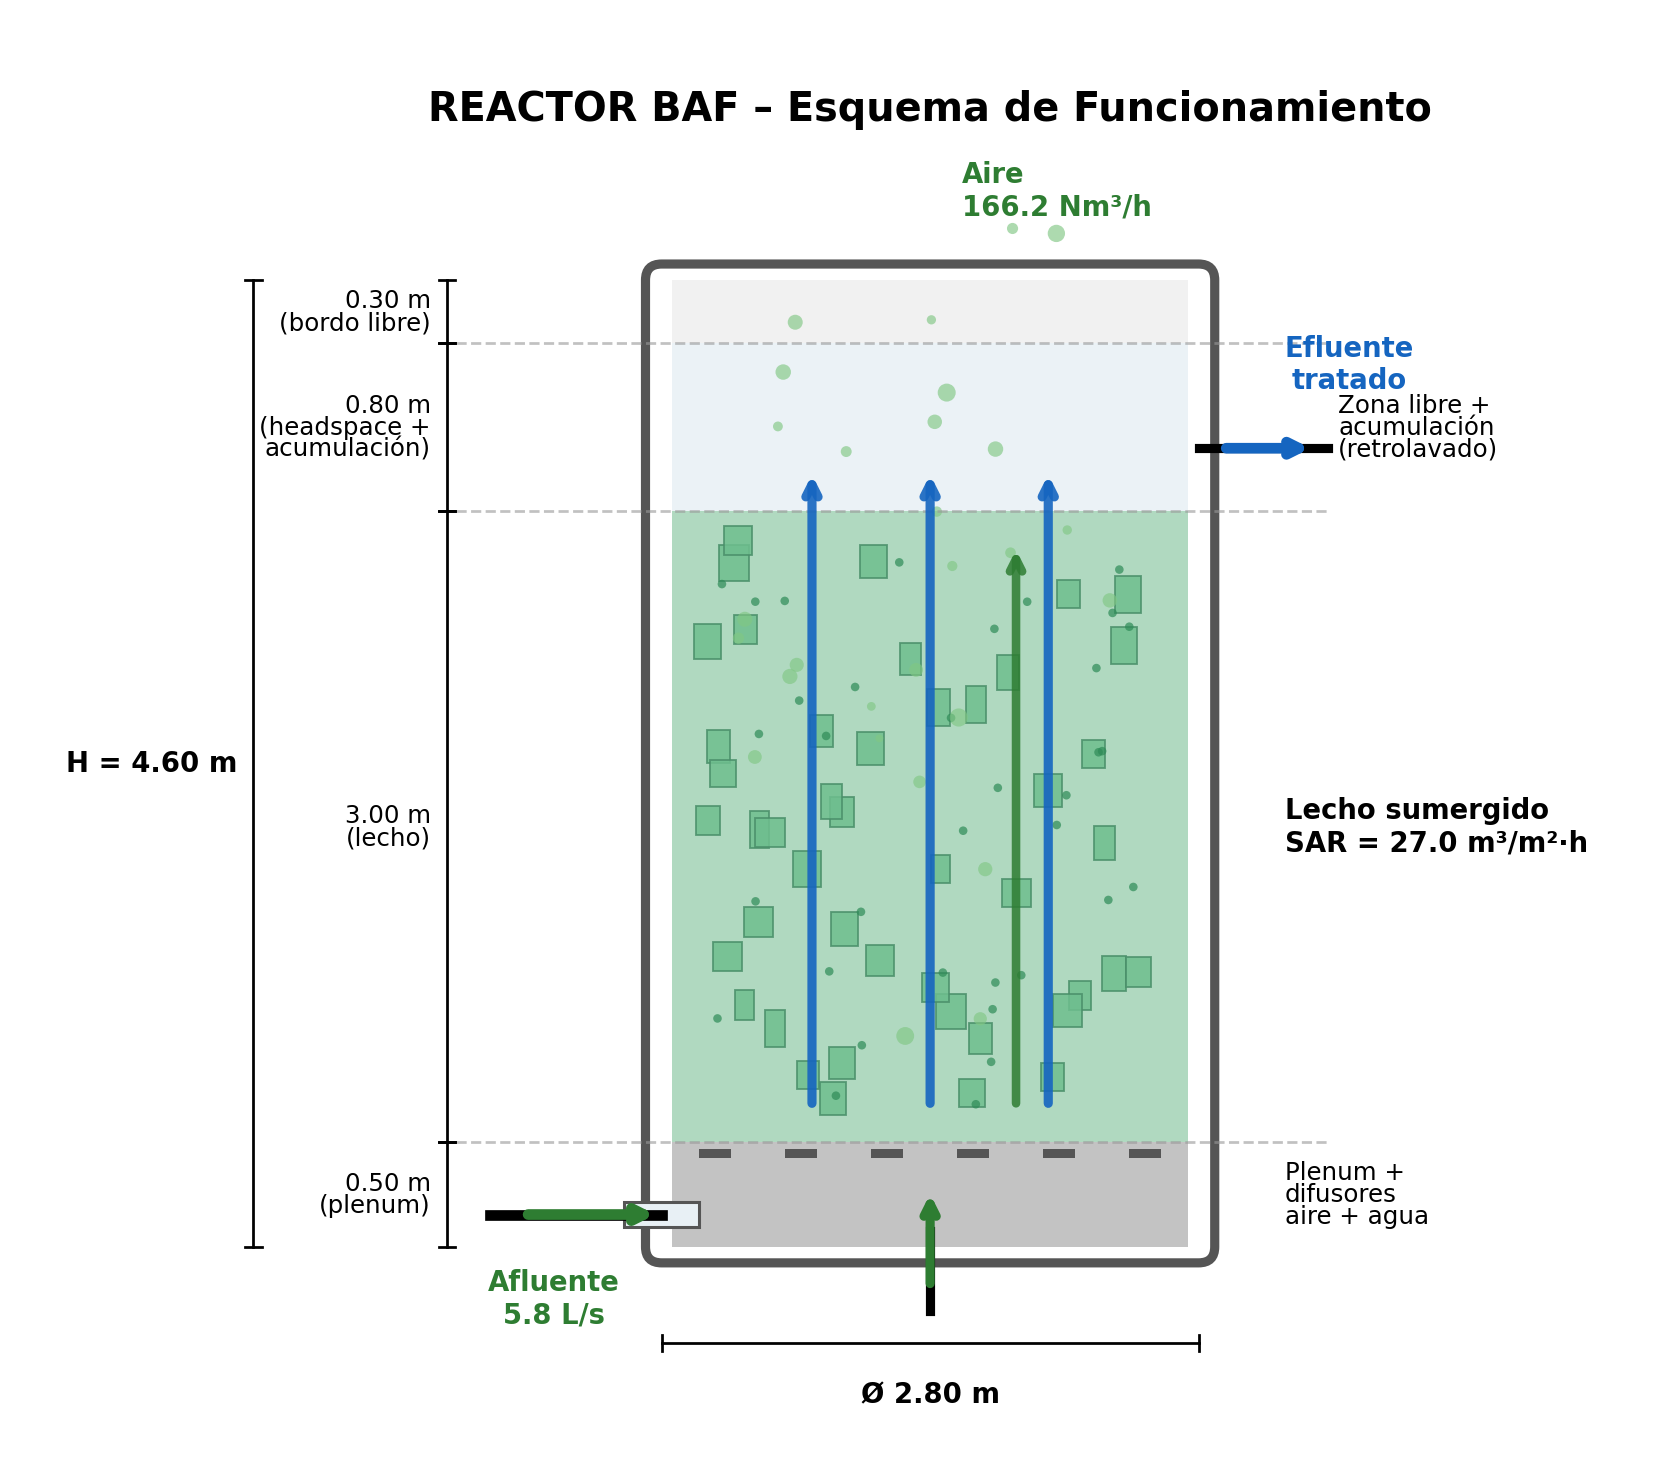
\includegraphics[width=0.75\textwidth]{figuras/Esquema_BAF.png}
\caption{Esquema del Biofiltro Biológico Aireado (BAF) -- vista vertical (sección transversal)}
\label{fig:esquema_baf}
\end{figure}

El esquema muestra la configuración de flujo ascendente (\textit{{up-flow}}) con aireación en co-corriente, el lecho de relleno plástico sumergido, y las zonas de plenum, headspace y acumulación para retrolavado.

\subsection{Sistema de Desinfeccion con Hipoclorito de Sodio}





La desinfección constituye la etapa final del proceso de tratamiento de aguas residuales, cuyo objetivo es la inactivación de microorganismos patógenos (bacterias, virus y protozoos) presentes en el efluente tratado, garantizando que su descarga al cuerpo receptor no represente riesgo para la salud pública ni para los ecosistemas acuáticos. En el contexto de la normativa ecuatoriana, la TULSMA (Texto Unificado de Legislación Secundaria del Ministerio del Ambiente) establece un límite máximo de 3000 NMP/100mL para coliformes fecales en vertimientos de aguas residuales tratadas.

El mecanismo de desinfección con compuestos clorados se fundamenta en la oxidación de componentes celulares esenciales de los microorganismos. El hipoclorito de sodio (NaOCl), al disolverse en agua, establece un equilibrio químico que genera ácido hipocloroso (HOCl) según la siguiente reacción:

\begin{equation}
\text{NaOCl} + \text{H}_2\text{O} \rightleftharpoons \text{HOCl} + \text{Na}^+ + \text{OH}^-
\end{equation}
\captionequation{Disolución del hipoclorito de sodio en agua}

El ácido hipocloroso (HOCl) es la especie biocida predominante y efectiva, siendo aproximadamente 80--100 veces más potente como desinfectante que el ion hipoclorito (OCl$^-$). La especiación entre HOCl y OCl$^-$ depende críticamente del pH del agua, según el siguiente equilibrio:

\begin{equation}
\text{HOCl} \rightleftharpoons \text{H}^+ + \text{OCl}^- \quad (\text{pKa} \approx 7,5 \text{ a 25°C})
\end{equation}
\captionequation{Equilibrio ácido-base del ácido hipocloroso}

A pH inferior a 7,5 predomina el HOCl (forma más efectiva), mientras que a pH superior a 7,5 predomina el OCl$^-$. Para el rango típico de pH de aguas residuales tratadas (6,5--8,5), se asegura una fracción significativa de HOCl que garantiza la eficacia desinfectante. La temperatura del agua también afecta este equilibrio: a mayor temperatura, el valor de pKa disminuye ligeramente, favoreciendo la forma HOCl.

\textbf{Mecanismos de inactivación microbiana}

La acción biocida del cloro se ejerce mediante múltiples mecanismos simultáneos: (1) \textit{oxidación de la pared celular}, alterando la permeabilidad y causando lisis celular; (2) \textit{denaturación de enzimas}, particularmente aquellas con grupos sulfhidrilo (-SH) que son oxidados a disulfuros; (3) \textit{daño al material genético}, mediante reacción con bases nitrogenadas del ADN y ARN; y (4) \textit{alteración del metabolismo celular}, inhibiendo la síntesis de ATP y otras funciones energéticas.

La susceptibilidad de los microorganismos al cloro varía significativamente. Las bacterias (incluyendo coliformes fecales) son generalmente las más susceptibles, con valores CT de 0,1--5 mg$\cdot$min/L para 2-log de reducción. Los virus requieren CT mayores (5--20 mg$\cdot$min/L), mientras que los protozoos como \textit{Giardia} y \textit{Cryptosporidium} son los más resistentes, requiriendo CT de 30--100 mg$\cdot$min/L o alternativas como UV o ozono.

\textbf{El concepto CT como parámetro de diseño}

El producto concentración-tiempo (CT) constituye el parámetro fundamental para el dimensionamiento de sistemas de desinfección. Fue desarrollado por la USEPA como criterio regulatorio y ha sido adoptado internacionalmente. Físicamente, el CT representa la exposición acumulada de los microorganismos al desinfectante, integrando tanto la concentración residual como el tiempo de contacto efectivo.

El CT requerido depende de: (a) el microorganismo objetivo y la reducción logarítmica deseada, (b) la temperatura del agua (a mayor temperatura, menor CT requerido debido a cinética más rápida), (c) el pH (afecta la especiación del cloro), y (d) la presencia de materia orgánica y otros consumidores de cloro (demanda).

Según Metcalf \& Eddy \cite{metcalf2014} y la USEPA \cite{usepa2003}, los valores CT típicos para inactivación de coliformes en efluentes secundarios son:

\begin{itemize}[noitemsep,leftmargin=2em]
    \item CT = 5--10 mg$\cdot$min/L: 2--3 log de reducción (99--99,9\%)
    \item CT = 10--20 mg$\cdot$min/L: 3--4 log de reducción (99,9--99,99\%)
    \item CT = 20--40 mg$\cdot$min/L: 4--5 log de reducción (99,99--99,999\%)
\end{itemize}

\textbf{Criterio de disenio basado en CF objetivo}

El dimensionamiento del sistema de desinfección se fundamenta en un criterio de diseño explícito basado en la concentración de coliformes fecales (CF) objetivo. A diferencia de un enfoque de dosis fija, este método garantiza que el sistema sea capaz de alcanzar el nivel de inactivación microbiológica requerido, partiendo de la carga de coliformes de entrada y definiendo la reducción logarítmica necesaria para cumplir con el objetivo de calidad del efluente.

Para este diseño, se establece un CF objetivo de 3000 NMP/100mL, correspondiente al límite establecido por la TULSMA para vertimiento de aguas residuales tratadas. Con una concentración de entrada de 715 NMP/100mL, la reducción logarítmica requerida es:

\begin{equation}
\text{Log reducción}_{\text{req}} = \log_{10}\left(\frac{CF_{\text{entrada}}}{CF_{\text{objetivo}}}\right) = \log_{10}\left(\frac{715}{3000}\right) = 0.00 \text{ log}
\end{equation}
\captionequation{Log reduccion requerida para cumplir CF objetivo}

El CT requerido para lograr esta reducción se calcula mediante el coeficiente de inactivación adoptado:

\begin{equation}
CT_{\text{req}} = \frac{\text{Log reducción}_{\text{req}}}{k} = \frac{0.00}{0.22} = 0.0 \text{ mg$\cdot$min/L}
\end{equation}
\captionequation{CT requerido para alcanzar la reduccion logaritmica objetivo}

\textbf{Filosofía de diseño adoptada: TRH base + Residual calculado}

El diseño adopta una filosofía de tiempo de contacto base y residual calculado. Primero se dimensiona el tanque de contacto con un TRH base de referencia (30 min), obteniéndose un TRH real de 53.7 min según las dimensiones constructivas adoptadas. Posteriormente, se calcula el residual requerido para alcanzar el CT objetivo con ese TRH real:

\begin{equation}
C_{\text{req}} = \frac{CT_{\text{req}}}{TRH_{\text{real}}} = \frac{0.0}{53.7} = 0.00 \text{ mg/L}
\end{equation}
\captionequation{Residual requerido para alcanzar CT objetivo con TRH real}

El residual adoptado corresponde al valor requerido calculado, optimizando la dosis para cumplir justo con el objetivo de desinfección:

\begin{equation}
C_{\text{adoptado}} = C_{\text{req}} = 0.56 \text{ mg/L}
\end{equation}
\captionequation{Residual adoptado para cumplir CF objetivo}

\textit{Nota operativa:} El residual calculado (0.00 mg/L) es inferior al mínimo operativo recomendado (0.5 mg/L) para garantizar margen de seguridad en la operación. Se recomienda monitorear periódicamente para asegurar que el residual efectivo se mantenga en el rango de 0,5--1,0 mg/L.

El CT real alcanzado con el residual adoptado y el TRH real es:

\begin{equation}
CT_{\text{real}} = C_{\text{adoptado}} \times TRH_{\text{real}} = 0.56 \times 53.7 = 30.0 \text{ mg$\cdot$min/L}
\end{equation}
\captionequation{CT real alcanzado}

Como criterio adicional de verificación, se establece un CT mínimo de 30 mg$\cdot$min/L, valor conservador que asegura el cumplimiento del límite de coliformes fecales establecido por la TULSMA, considerando las variaciones operativas esperadas.

\textbf{Demanda de cloro y dosificación}

La demanda de cloro representa la cantidad de cloro consumida por reacciones con sustancias presentes en el agua antes de que quede disponible cloro residual libre para desinfección. Los principales consumidores son: amoníaco (formando cloraminas), materia orgánica reducida, compuestos férricos y manganesos, y sulfuros. En efluentes secundarios tratados (post-filtro percolador), la demanda típica adoptada para referencia de diseño varía entre 2--5 mg/L dependiendo de la calidad del efluente.

El cloro residual es la concentración que permanece después de satisfacer la demanda y es la que ejerce el efecto desinfectante. El diseño debe garantizar un residual mínimo de 0.6 mg/L al final del tiempo de contacto para asegurar eficacia. La dosis total a aplicar es:

\begin{equation}
\text{Dosis total} = \text{Demanda} + \text{Residual objetivo}
\end{equation}
\captionequation{Descomposición de la dosis de cloro}

\textbf{Diseño del tanque de contacto}

El tanque de contacto se dimensiona para proporcionar un tiempo de retención hidráulico (TRH) adecuado que permita alcanzar el CT objetivo con el residual calculado. El TRH efectivo es el tiempo que permanece el agua en el tanque, calculado como el cociente entre el volumen útil y el caudal. Según Metcalf \& Eddy, para desinfección de efluentes secundarios se recomienda un TRH de 15--45 min; para este caso, se parte de un TRH base de 30 min para el dimensionamiento geométrico.

La geometría del tanque debe favorecer el flujo en pistón (plug flow) para evitar cortocircuitos hidráulicos que reduzcan el tiempo efectivo de contacto. Por ello, el volumen de contacto se organiza como una cámara con bafles alternados tipo culebrín, de modo que el recorrido hidráulico aumente y la relación recorrido/ancho del canal sea verificable.

\textbf{Parámetros de diseño adoptados}

El sistema se dimensiona considerando los siguientes parámetros fundamentales, establecidos según criterios bibliográficos y normativos:

\begin{table}[H]
\centering
\caption{Parámetros de diseño de la desinfección}
\small
\begin{tabular}{@{}p{0.28\textwidth}p{0.18\textwidth}p{0.22\textwidth}p{0.18\textwidth}@{}}
\toprule
\textbf{Parámetro} & \textbf{Valor adoptado} & \textbf{Rango/Unidad} & \textbf{Fuente} \\
\midrule
Demanda de cloro & 3.5 mg/L & 2--5 mg/L & Estimado efluente post-sedimentador \\
Residual requerido & 0.00 mg/L & -- & Cálculo desde CT \\
Residual adoptado & 0.56 mg/L & $>$0.00 mg/L & Para cumplir CF objetivo \\
Dosis total & 4.1 mg/L & 3--10 mg/L & Metcalf \& Eddy \cite{metcalf2014} \\
TRH base de diseño & 30 min & 15--45 min & Configuración \\
TRH real del tanque & 53.7 min & $\geq$ 30 min & Dimensionado \\
Relación recorrido/ancho & 30.0:1 & $\geq$ 30:1 & Criterio de flujo pistón \\
CT requerido & 0.0 mg$\cdot$min/L & -- & Desde log reducción \\
CT real & 30.0 mg$\cdot$min/L & $\geq$ 30 mg$\cdot$min/L & Residual $\times$ TRH \\
\bottomrule
\end{tabular}
\end{table}

La dosis total de cloro se descompone en la demanda del efluente (consumida por amoníaco y materia orgánica) más el residual requerido para desinfección:

\begin{equation}
\text{Dosis total} = \text{Demanda} + \text{Residual} = 3.5 + 0.6 = 4.1 \text{ mg/L}
\end{equation}
\captionequation{Dosis total de cloro}

\textbf{Cálculo del producto CT}

La eficacia de la desinfección se cuantifica mediante el parámetro CT:

\begin{equation}
CT = C \times t
\end{equation}
\captionequation{Producto concentracion-tiempo CT}

\textit{Donde:}
\begin{itemize}[noitemsep,leftmargin=2em]
    \item[$CT$] = Producto concentración-tiempo (mg$\cdot$min/L)
    \item[$C$] = Cloro residual (0.6 mg/L)
    \item[$t$] = Tiempo de contacto real en la cámara (53.7 min)
\end{itemize}

\begin{equation}
CT = 0.56 \times 53.7 = 30.0 \text{ mg$\cdot$min/L}
\end{equation}

La reducción de coliformes se estima mediante una relación empírica simplificada, válida como aproximación preliminar de diseño para efluentes secundarios típicos:

\begin{equation}
\text{Log reducción} \approx 0.22 \times CT
\end{equation}
\captionequation{Estimacion empirica de log-reduccion (simplificacion para diseño preliminar)}

\textit{Nota metodológica:} Esta relación lineal es una simplificación empírica calibrada para condiciones típicas de aguas residuales tratadas (pH 6.5--8.5, temperatura 20--25°C, baja materia orgánica residual). El modelo cinético formal de inactivación microbiana es el de Chick-Watson: $N/N_0 = e^{-k \cdot C^n \cdot t}$, donde $k$ es la constante de inactivación específica para cada microorganismo y $n$ es el coeficiente de dilución (típicamente $n \approx 1$ para cloro libre). La forma lineal utilizada es práctica para diseño preliminar pero debe verificarse con ensayos de desinfección específicos si se requiere precisión rigurosa.

\begin{equation}
\text{Log reducción} \approx 0.22 \times 30 = 6.6 \text{ log}
\end{equation}

Los coliformes finales se calculan como:

\begin{equation}
CF_{final} = \frac{CF_{inicial}}{10^{\text{Log reduccion}}} = \frac{715}{10^{6.6}} = 0 \text{ NMP/100mL}
\end{equation}

\textbf{Dimensionamiento del tanque de contacto}

El volumen del tanque se determina por:

\begin{equation}
V = Q \times t
\end{equation}
\captionequation{Volumen del tanque de contacto}

\textit{Donde:}
\begin{itemize}[noitemsep,leftmargin=2em]
    \item[$V$] = Volumen del tanque (m³)
    \item[$Q$] = Caudal (498.5 m³/d = 0.346 m³/min)
    \item[$t$] = Tiempo de contacto base (30 min)
\end{itemize}

\begin{equation}
V_{min} = 0.346 \times 30 = 10.4 \text{ m}^3
\end{equation}

El volumen minimo por tiempo de contacto es 10.4 m3; la geometria serpentina adoptada entrega 18.6 m3 y un tiempo hidraulico teorico de 53.7 min.

La cámara se resuelve con 5 canales en culebrín, ancho hidráulico de 0.50 m por canal, bafles de 0.15 m y un recorrido hidráulico total de 15.0 m. Las dimensiones en planta resultantes son 3.0 m de largo por 3.1 m de ancho.

\textbf{Consumo de cloro y requerimientos de producto comercial}

El consumo de cloro activo (como Cl$_2$) se calcula como:

\begin{equation}
\text{Consumo Cl}_2 = \frac{D \times Q}{1000} = \frac{4.1 \times 498.5}{1000} = 2.02 \text{ kg Cl}_2\text{/d}
\end{equation}

\textbf{Conversión a hipoclorito de sodio comercial (NaOCl):}

El hipoclorito de sodio se comercializa típicamente al 10--12.5\% de cloro disponible. La conversión se realiza mediante:

\begin{equation}
\text{Consumo NaOCl} = \frac{\text{Consumo Cl}_2}{[\% \text{ NaOCl}]} = \frac{2.02}{10\%} = 20.2 \text{ kg NaOCl/d}
\end{equation}
\captionequation{Conversion a hipoclorito de sodio comercial}

Considerando una densidad de 1.10 kg/L para la solución al 10\%:

\begin{equation}
\text{Volumen NaOCl} = \frac{20.2 \text{ kg/d}}{1.10 \text{ kg/L}} = 18.4 \text{ L/d} \approx 552 \text{ L/mes}
\end{equation}

El volumen de almacenamiento en bodega se recomienda para 30 días de operación: 552 L (equivalente a 0.6 m³).

\textbf{Nota sobre subproductos de la desinfección}

La cloración de aguas residuales puede generar subproductos de desinfección (DBPs, por sus siglas en inglés), principalmente trihalometanos (THMs) y ácidos haloacéticos (HAAs), como resultado de la reacción del cloro con la materia orgánica residual presente en el efluente tratado.

Para plantas de tratamiento de pequeña escala como la proyectada, la formación de THMs puede controlarse mediante cuatro medidas operativas integrales. En primer lugar, el control de dosis debe enfocarse en aplicar la dosis mínima efectiva que garantice el residual requerido, evitando sobredosis innecesaria que incrementaría la generación de subproductos. En segundo lugar, el monitoreo de residual combinado debe mantenerse en el rango de 0.6--1.0 mg/L, ya que valores superiores favorecen la formación de DBPs. En tercer lugar, la calidad del efluente previo resulta determinante: asegurar que el tratamiento biológico previo (HAFV) remueva adecuadamente la materia orgánica reduce el potencial de formación de THMs, dado que una menor DQO/DBO residual implica menor disponibilidad de precursores orgánicos. Finalmente, el monitoreo periódico mediante análisis trimestral de THMs totales en el efluente final debe realizarse si la autoridad ambiental lo requiere; para vertimiento a cuerpos receptores no destinados a consumo humano, los requisitos normativos son menos estrictos que para agua potable.

Para el presente diseño, el riesgo de formación de THMs se considera manejable mediante la operación adecuada del sistema de dosificación y el control de residual, dado que el efluente del HAFV tiene baja concentración de materia orgánica precursora y la dosis de cloro aplicada es moderada.

\subsubsection{Verificación}

\textbf{Verificación de cumplimiento normativo}

El sistema de desinfección se verifica contra los criterios establecidos en la TULSMA y las recomendaciones de Metcalf \& Eddy para asegurar la eficacia del proceso.


El Texto Unificado de Legislación Secundaria del Ministerio del Ambiente (TULSMA) establece diferentes límites de coliformes fecales según el uso receptor del agua. La siguiente tabla compara el valor calculado de coliformes finales (0 NMP/100mL) con los límites establecidos para cada categoría de uso:

\begin{table}[H]
\centering
\caption{Comparación con límites TULSMA por uso del agua}
\small
\begin{tabular}{@{}llcc@{}}
\toprule
\textbf{Uso / Tabla TULSMA} & \textbf{CF (límite)} & \textbf{CF calculado} & \textbf{Dictamen} \\
\midrule
Agua dulce -- Tabla 12 & $\leq$3000 & 0 & \textbf{CUMPLE} \\
Agua marina -- Tabla 13 & $\leq$3000 & 0 & \textbf{CUMPLE} \\
Alcantarillado -- Tabla 11 & --- & 0 & \textbf{N/A} \\
Flora y fauna -- Tabla 3 & $\leq$200 & 0 & \textbf{CUMPLE} \\
Agrícola/riego -- Tabla 6 & $\leq$1000 & 0 & \textbf{CUMPLE} \\
Pecuario -- Tabla 7 & $\leq$1000 & 0 & \textbf{CUMPLE} \\
Recreativo primario -- Tabla 9 & $\leq$200 & 0 & \textbf{CUMPLE} \\
Recreativo secundario -- Tabla 10 & $\leq$2000 & 0 & \textbf{CUMPLE} \\
Consumo humano -- Tabla 1 & $\leq$600 & 0 & \textbf{CUMPLE} \\
\bottomrule
\end{tabular}
\end{table}

Cumple con el límite de TULSMA (CF final = 0 NMP/100mL $≤$ 3000 NMP/100mL).

El producto CT es indicativo de la eficacia de la desinfección. Un valor CT adecuado garantiza la reducción suficiente de microorganismos patógenos.

\begin{table}[H]
\centering
\caption{Verificación del producto CT}
\begin{tabular}{@{}lcc@{}}
\toprule
\textbf{Parámetro} & \textbf{Valor calculado} & \textbf{Valor recomendado} \\
\midrule
CT calculado & 30 mg$\cdot$min/L & $\geq$ 30 mg$\cdot$min/L \\
Estado & \multicolumn{2}{c}{\textbf{Cumple}} \\
\bottomrule
\end{tabular}
\end{table}

El valor CT real (30.0 mg$⋅$min/L) supera el mínimo recomendado de 30 mg$⋅$min/L.


\textbf{Notas de operación}

Se recomienda monitorear el cloro residual en la salida del tanque (debe mantenerse entre 0,5--1,0 mg/L) y ajustar la dosis según la demanda del efluente. Realizar pruebas de coliformes periódicas para verificar la eficacia del sistema.

La reducción logarítmica alcanzada es de 6.6 log, lo que representa una reducción porcentual del 100.0\% de los coliformes presentes en el efluente.

\subsubsection{Resultados}

\begingroup
\small
\begin{longtable}{@{}lc@{}}
\caption{Resumen de dimensiones y parámetros de la desinfección}\\
\toprule
\textbf{Parámetro} & \textbf{Valor} \\
\midrule
\endfirsthead
\caption[]{Resumen de dimensiones y parámetros de la desinfección (continuación)}\\
\toprule
\textbf{Parámetro} & \textbf{Valor} \\
\midrule
\endhead
\midrule
\multicolumn{2}{r}{\textit{Continúa en la siguiente página}} \\
\endfoot
\bottomrule
\endlastfoot
\multicolumn{2}{l}{\textit{Dimensiones del tanque}} \\
\midrule
Largo & 3.0 m \\
Ancho & 3.1 m \\
Canales del culebrin & 5 pasos de 0.50 m \\
Recorrido hidraulico & 15.0 m (30.0:1) \\
Profundidad útil & 2.0 m \\
Altura total & 2.30 m \\
Volumen útil & 18.6 m³ \\
\midrule
\multicolumn{2}{l}{\textit{Parámetros de desinfección}} \\
\midrule
Demanda de cloro & 3.5 mg/L \\
Cloro residual & 0.6 mg/L \\
Dosis total & 4.1 mg/L \\
TRH base & 30 min \\
TRH real & 53.7 min \\
CT & 30 mg$\cdot$min/L \\
Log reducción & 6.6 log \\
CF final & 0 NMP/100mL \\
\midrule
\multicolumn{2}{l}{\textit{Consumo de productos}} \\
\midrule
Consumo Cl$_2$ activo & 2.02 kg/d \\
Concentración NaOCl & 10 \% \\
Consumo NaOCl & 20.2 kg/d \\
Volumen NaOCl & 18.4 L/d (552 L/mes) \\
Almacenamiento (30 d) & 552 L (0.6 m³) \\
\end{longtable}
\endgroup

El sistema de desinfección con hipoclorito de sodio ha sido dimensionado para tratar un caudal de 498.5 m³/d, logrando una reducción de 100.0\% de coliformes fecales. El cumplimiento respecto a los límites de la TULSMA depende de la categoría de uso receptor específica del proyecto, conforme al dictamen técnico presentado en la tabla de verificación anterior.\

\begin{figure}[H]
\centering

\includegraphics[width=0.95\textwidth]{figuras/Esquema_Camara_Contacto_Cloro.png}
\caption{Cámara de contacto de cloración tipo culebrín: planta con bafles alternados y sección transversal. Recorrido hidráulico: 15.0 m; relación recorrido/ancho: 30.0:1; volumen útil adoptado: 18.6 m³.}
\label{fig:camara_contacto_cloro}
\end{figure}



La camara de contacto se configura como culebrin con 5 pasos hidraulicos, ancho de canal de 0.50 m y recorrido total de 15.0 m. La relacion recorrido/ancho es 30.0:1, frente al criterio minimo adoptado de 30:1 para aproximar flujo piston y reducir cortocircuitos hidraulicos. El estado de la verificacion es Cumple.



\subsection{Lechos de Secado de Lodos}

\subsubsection{Lechos de Secado de Lodos}
Error: 't_secado_d'




\newpage
\bibliographystyle{plain}
\bibliography{referencias}


\newpage
\appendix
\section{Anexo: TULSMA -- Criterios de Calidad del Recurso Agua}
\label{app:tulsma}

\begin{center}
{\LARGE\bfseries TULSMA -- Norma de Calidad Ambiental\\[4pt]
del Recurso Agua}\\[8pt]
{\large Libro VI, Anexo 1 -- Acuerdo Ministerial 097-A (2015)\\
Decreto Ejecutivo 3516 -- Ecuador}\\[4pt]
{\small Criterios de calidad por uso del agua y limites de descarga de efluentes}
\end{center}
\vspace{10pt}

\subsection{Tabla 1 -- Consumo Humano y Uso Domestico (tratamiento convencional)}
\small
\begin{longtable}{p{4.5cm}p{2.0cm}p{2.0cm}p{3.5cm}}
\caption{Limites maximos permisibles para aguas de consumo humano y uso domestico que unicamente requieren tratamiento convencional (TULSMA, Tabla~1).}\\
\toprule
\textbf{Parametro} & \textbf{Expresado como} & \textbf{Unidad} & \textbf{Limite maximo permisible} \\
\midrule
\endfirsthead
\multicolumn{4}{c}{\small\itshape Continuacion de la Tabla}\\
\toprule
\textbf{Parametro} & \textbf{Expresado como} & \textbf{Unidad} & \textbf{Limite maximo permisible} \\
\midrule
\endhead
\bottomrule
\endlastfoot
Aceites y Grasas & Sust.\ solubles en hexano & mg/L & $\leq$ 0,3 \\
Aluminio & Al & mg/L & $\leq$ 0,2 \\
Amoniaco & N-Amoniacal & mg/L & $\leq$ 1,0 \\
Amonio & NH$_4$ & mg/L & $\leq$ 0,05 \\
Arsenico (total) & As & mg/L & $\leq$ 0,05 \\
Bario & Ba & mg/L & $\leq$ 1,0 \\
Cadmio & Cd & mg/L & $\leq$ 0,01 \\
Cianuro total & CN$^-$ & mg/L & $\leq$ 0,1 \\
Cloruros & Cl$^-$ & mg/L & $\leq$ 250 \\
Cobre & Cu & mg/L & $\leq$ 1,0 \\
\textbf{Coliformes totales} & NMP & NMP/100 mL & $\leq$ 3\,000 \\
\textbf{Coliformes fecales} & NMP & NMP/100 mL & $\leq$ 600 \\
Color real & UC & Unidades de color & $\leq$ 100 \\
Compuestos fenolicos & Fenol & mg/L & $\leq$ 0,002 \\
Cromo hexavalente & Cr$^{6+}$ & mg/L & $\leq$ 0,05 \\
\textbf{DBO$_5$} & -- & mg/L & $\leq$ 2,0 \\
Dureza & CaCO$_3$ & mg/L & $\leq$ 500 \\
Fluoruro total & F & mg/L & $\leq$ 1,5 \\
Hierro total & Fe & mg/L & $\leq$ 1,0 \\
Manganeso total & Mn & mg/L & $\leq$ 0,1 \\
Materia flotante & -- & -- & Ausencia \\
Mercurio total & Hg & mg/L & $\leq$ 0,001 \\
Nitrato & N-Nitrato & mg/L & $\leq$ 10,0 \\
Nitrito & N-Nitrito & mg/L & $\leq$ 1,0 \\
Oxigeno disuelto & O.D. & mg/L & $\geq$ 80\% saturacion; $\geq$ 6 mg/L \\
pH & -- & -- & $6,0 - 9,0$ \\
Plata total & Ag & mg/L & $\leq$ 0,05 \\
Plomo total & Pb & mg/L & $\leq$ 0,05 \\
Selenio total & Se & mg/L & $\leq$ 0,01 \\
Sodio & Na & mg/L & $\leq$ 200 \\
Solidos disueltos totales & -- & mg/L & $\leq$ 1\,000 \\
Sulfatos & SO$_4^{2-}$ & mg/L & $\leq$ 400 \\
Temperatura & -- & $^\circ$C & Cond.\ natural $\pm$ 3\,$^\circ$C \\
Tensoactivos & SAAM & mg/L & $\leq$ 0,5 \\
Turbiedad & -- & UTN & $\leq$ 100 \\
Zinc & Zn & mg/L & $\leq$ 5,0 \\
\end{longtable}

\subsection{Tabla 12 -- Descarga a Cuerpo de Agua Dulce}
{\small\textbf{Nota:} Esta es la tabla aplicable al proyecto de tratamiento de aguas residuales municipales cuando el efluente se vierte a un rio, lago o cuerpo superficial de agua dulce.}
\vspace{6pt}
\small
\begin{longtable}{p{4.5cm}p{2.0cm}p{2.0cm}p{3.5cm}}
\caption{Limites maximos permisibles de descarga a un cuerpo de agua dulce (TULSMA, Tabla~12).}\\
\toprule
\textbf{Parametro} & \textbf{Expresado como} & \textbf{Unidad} & \textbf{Limite maximo permisible} \\
\midrule
\endfirsthead
\multicolumn{4}{c}{\small\itshape Continuacion de la Tabla}\\
\toprule
\textbf{Parametro} & \textbf{Expresado como} & \textbf{Unidad} & \textbf{Limite maximo permisible} \\
\midrule
\endhead
\bottomrule
\endlastfoot
Aceites y grasas & Sust.\ solubles en hexano & mg/L & $\leq$ 0,3 \\
Aluminio & Al & mg/L & $\leq$ 5,0 \\
Arsenico total & As & mg/L & $\leq$ 0,1 \\
Bario & Ba & mg/L & $\leq$ 2,0 \\
Cadmio & Cd & mg/L & $\leq$ 0,02 \\
Cianuro total & CN$^-$ & mg/L & $\leq$ 0,1 \\
Cloruros & Cl$^-$ & mg/L & $\leq$ 1\,000 \\
Cobre & Cu & mg/L & $\leq$ 1,0 \\
\textbf{Coliformes fecales}$^\dagger$ & NMP & NMP/100 mL & $\leq$ 3\,000 \\
Compuestos fenolicos & Fenol & mg/L & $\leq$ 0,2 \\
Cromo hexavalente & Cr$^{6+}$ & mg/L & $\leq$ 0,5 \\
\textbf{DBO$_5$} & -- & mg/L & $\leq$ 100 \\
\textbf{DQO} & -- & mg/L & $\leq$ 250 \\
Fluoruros & F$^-$ & mg/L & $\leq$ 5,0 \\
Fosforo total & P & mg/L & $\leq$ 10,0 \\
Hierro total & Fe & mg/L & $\leq$ 10,0 \\
Manganeso total & Mn & mg/L & $\leq$ 2,0 \\
Materia flotante & -- & -- & Ausencia \\
Mercurio total & Hg & mg/L & $\leq$ 0,005 \\
Niquel & Ni & mg/L & $\leq$ 2,0 \\
Nitrogeno amoniacal & N-NH$_3$ & mg/L & $\leq$ 30,0 \\
Nitrogeno total Kjeldahl & N-TKN & mg/L & $\leq$ 50,0 \\
pH & -- & -- & $6,0 - 9,0$ \\
Plata total & Ag & mg/L & $\leq$ 0,1 \\
Plomo total & Pb & mg/L & $\leq$ 0,2 \\
Selenio & Se & mg/L & $\leq$ 0,1 \\
\textbf{Solidos sedimentables} & -- & mL/L & $\leq$ 1,0 \\
\textbf{Solidos suspendidos totales} & -- & mg/L & $\leq$ 130 \\
Solidos totales & -- & mg/L & $\leq$ 1\,600 \\
Sulfatos & SO$_4^{2-}$ & mg/L & $\leq$ 1\,000 \\
Sulfuros & S$^{2-}$ & mg/L & $\leq$ 0,5 \\
Temperatura & -- & $^\circ$C & Cond.\ natural $\pm$ 3\,$^\circ$C; max.\ 32\,$^\circ$C \\
Tensoactivos & SAAM & mg/L & $\leq$ 0,5 \\
Zinc & Zn & mg/L & $\leq$ 5,0 \\
\multicolumn{4}{l}{\scriptsize $^\dagger$ Aquellos con descargas $\leq$ 3\,000 NMP/100 mL quedan exentos de tratamiento de desinfeccion.}\\
\end{longtable}
\normalsize

\subsection{Tabla 13 -- Descarga a Cuerpo de Agua Marina}
\small
\begin{longtable}{p{4.5cm}p{2.0cm}p{2.0cm}p{3.5cm}}
\caption{Limites maximos permisibles de descarga a un cuerpo de agua marina (TULSMA, Tabla~13).}\\
\toprule
\textbf{Parametro} & \textbf{Expresado como} & \textbf{Unidad} & \textbf{Limite maximo permisible} \\
\midrule
\endfirsthead
\multicolumn{4}{c}{\small\itshape Continuacion de la Tabla}\\
\toprule
\textbf{Parametro} & \textbf{Expresado como} & \textbf{Unidad} & \textbf{Limite maximo permisible} \\
\midrule
\endhead
\bottomrule
\endlastfoot
Aceites y grasas & Sust.\ solubles en hexano & mg/L & $\leq$ 0,3 \\
Aluminio & Al & mg/L & $\leq$ 5,0 \\
Arsenico total & As & mg/L & $\leq$ 0,1 \\
Cadmio & Cd & mg/L & $\leq$ 0,1 \\
Cianuro total & CN$^-$ & mg/L & $\leq$ 0,1 \\
Cobre & Cu & mg/L & $\leq$ 0,5 \\
\textbf{Coliformes fecales}$^\ddagger$ & NMP & NMP/100 mL & $\leq$ 3\,000 \\
Compuestos fenolicos & Fenol & mg/L & $\leq$ 0,2 \\
Cromo hexavalente & Cr$^{6+}$ & mg/L & $\leq$ 0,5 \\
\textbf{DBO$_5$} & -- & mg/L & $\leq$ 100 \\
\textbf{DQO} & -- & mg/L & $\leq$ 250 \\
Fluoruros & F$^-$ & mg/L & $\leq$ 5,0 \\
Hierro total & Fe & mg/L & $\leq$ 10,0 \\
Manganeso total & Mn & mg/L & $\leq$ 2,0 \\
Materia flotante & -- & -- & Ausencia \\
Mercurio total & Hg & mg/L & $\leq$ 0,005 \\
Niquel & Ni & mg/L & $\leq$ 2,0 \\
Nitrogeno amoniacal & N-NH$_3$ & mg/L & $\leq$ 30,0 \\
Nitrogeno total Kjeldahl & N-TKN & mg/L & $\leq$ 50,0 \\
pH & -- & -- & $6,0 - 9,0$ \\
Plomo total & Pb & mg/L & $\leq$ 0,2 \\
\textbf{Solidos suspendidos totales} & -- & mg/L & $\leq$ 100 \\
Temperatura & -- & $^\circ$C & Cond.\ natural $\pm$ 3\,$^\circ$C; max.\ 32\,$^\circ$C \\
Tensoactivos & SAAM & mg/L & $\leq$ 0,5 \\
Zinc & Zn & mg/L & $\leq$ 5,0 \\
\multicolumn{4}{l}{\footnotesize $^\ddagger$ Aquellos con descargas $\leq$ 3\,000 NMP/100 mL quedan exentos de tratamiento de desinfeccion.}\\
\end{longtable}

\subsection{Tabla 11 -- Descarga al Sistema de Alcantarillado Publico}
\small
\begin{longtable}{p{4.5cm}p{2.0cm}p{2.0cm}p{3.5cm}}
\caption{Limites maximos permisibles de descarga al sistema de alcantarillado publico (TULSMA, Tabla~11).}\\
\toprule
\textbf{Parametro} & \textbf{Expresado como} & \textbf{Unidad} & \textbf{Limite maximo permisible} \\
\midrule
\endfirsthead
\multicolumn{4}{c}{\small\itshape Continuacion de la Tabla}\\
\toprule
\textbf{Parametro} & \textbf{Expresado como} & \textbf{Unidad} & \textbf{Limite maximo permisible} \\
\midrule
\endhead
\bottomrule
\endlastfoot
Aceites y grasas & Sust.\ solubles en hexano & mg/L & $\leq$ 70,0 \\
Aluminio & Al & mg/L & $\leq$ 5,0 \\
Arsenico total & As & mg/L & $\leq$ 0,1 \\
Bario & Ba & mg/L & $\leq$ 2,0 \\
Cadmio & Cd & mg/L & $\leq$ 0,02 \\
Cianuro total & CN$^-$ & mg/L & $\leq$ 1,0 \\
Cloruros & Cl$^-$ & mg/L & $\leq$ 1\,000 \\
Cobre & Cu & mg/L & $\leq$ 1,0 \\
Coliformes fecales & NMP & NMP/100 mL & No especificado \\
Compuestos fenolicos & Fenol & mg/L & $\leq$ 0,2 \\
Cromo hexavalente & Cr$^{6+}$ & mg/L & $\leq$ 0,5 \\
Cromo total & Cr & mg/L & $\leq$ 0,5 \\
\textbf{DBO$_5$} & -- & mg/L & $\leq$ 250 \\
\textbf{DQO} & -- & mg/L & $\leq$ 500 \\
Fluoruros & F$^-$ & mg/L & $\leq$ 5,0 \\
Hierro total & Fe & mg/L & $\leq$ 25,0 \\
Manganeso total & Mn & mg/L & $\leq$ 10,0 \\
Materia flotante & -- & -- & Ausencia \\
Mercurio total & Hg & mg/L & $\leq$ 0,01 \\
Niquel & Ni & mg/L & $\leq$ 2,0 \\
Nitrogeno amoniacal & N-NH$_3$ & mg/L & $\leq$ 30,0 \\
pH & -- & -- & $6,0 - 9,0$ \\
Plata total & Ag & mg/L & $\leq$ 0,5 \\
Plomo total & Pb & mg/L & $\leq$ 0,5 \\
Selenio & Se & mg/L & $\leq$ 0,5 \\
\textbf{Solidos sedimentables} & -- & mL/L/h & $\leq$ 20 \\
\textbf{Solidos suspendidos totales} & -- & mg/L & $\leq$ 220 \\
Sulfatos & SO$_4^{2-}$ & mg/L & $\leq$ 1\,000 \\
Sulfuros & S$^{2-}$ & mg/L & $\leq$ 1,0 \\
Temperatura & -- & $^\circ$C & $\leq$ 40 \\
Tensoactivos & SAAM & mg/L & $\leq$ 2,0 \\
Zinc & Zn & mg/L & $\leq$ 5,0 \\
\end{longtable}

\end{document}